% =========================================================================
% Beyond Closed-Set Accuracy: Constituent-Level Generalization in Compound
% Motor Fault Diagnosis
%
% Reconstructed, complete manuscript. Compiled here with the IEEEtran
% journal class as a stand-in for the IEEE Access template class
% (ieeeaccess.cls); the section files are template-agnostic, so moving them
% into the official template is mechanical: copy sections/, refs.bib and
% figures/, and transplant the \author block into the template's own
% front-matter macros.
%
% Build: pdflatex main && bibtex main && pdflatex main && pdflatex main
% =========================================================================
\documentclass[journal]{IEEEtran}

\usepackage[utf8]{inputenc}
\usepackage[T1]{fontenc}
\usepackage{amsmath,amssymb,amsfonts}
\usepackage{graphicx}
\usepackage{makecell}
\usepackage{booktabs}
\usepackage{url}
\graphicspath{{figures/}}

% Notation used throughout
\newcommand{\Fmicro}{F_{1,\mathrm{micro}}}
\newcommand{\Factive}{F_{1,\mathrm{active}}}

\begin{document}

\title{Beyond Closed-Set Accuracy: Constituent-Level Generalization in
Compound Motor Fault Diagnosis}

\author{Evin~\c{S}ahin~Sad{\i}k,
        H\"useyin~Tayyer~Canseven,~\IEEEmembership{Member,~IEEE}%
\thanks{Evin \c{S}ahin Sad{\i}k is with the Department of Electrical and
Electronics Engineering, K\"utahya Dumlup{\i}nar University, 43100
K\"utahya, Turkey (e-mail: evin.sahin@dpu.edu.tr).}%
\thanks{H\"useyin Tayyer Canseven is with the Department of Electrical
Engineering, Lappeenranta-Lahti University of Technology (LUT University),
53850 Lappeenranta, Finland (e-mail: huseyin.canseven@lut.fi).}%
\thanks{Corresponding author: H\"useyin Tayyer Canseven.}%
\thanks{This work was supported by the Academy of Finland under the Centre
of Excellence Programme for the project High-Speed Electromechanical Energy
Conversion Systems.}}

\markboth{IEEE Access}%
{\c{S}ahin Sad{\i}k \MakeLowercase{\textit{et al.}}: Beyond Closed-Set
Accuracy: Constituent-Level Generalization in Compound Motor Fault
Diagnosis}

\maketitle

\begin{abstract}
Reported accuracies for data-driven motor fault diagnosis are frequently
near ceiling, yet they rarely measure the ability that industrial deployment
actually requires: recognizing the elementary fault mechanisms of a compound
fault whose exact combination was never observed during model development.
This paper evaluates that ability on a public multimodal dataset of a 2.2-kW
three-phase induction motor containing 24 diagnostic states, including nine
compound faults that pair a mechanical bearing defect with a second
mechanical, electrical, or electromagnetic mechanism, under twelve
speed/load conditions. The problem is formulated at the constituent level:
nine elementary mechanisms are detected independently from physics-guided,
mechanism-specific vibration- and current-domain features, so unseen
combinations remain expressible. A crossed protocol separates three levels
of compound-context exposure (recombination, one-sided, and two-sided
context zero-shot) from operating-condition novelty, with run-level,
severity-aware splits and all calibration confined to training data.
Although closed-set 24-class accuracy reaches 0.913, exact recovery of
unseen constituent sets remains between 0.083 and 0.157 for the locked
linear probe, and every metric is reported against input-independent
prevalence references that expose partial-recovery scores as otherwise
misleading. Compound-context deprivation is measurably harmful chiefly when
the operating condition is also unseen (micro-$F_1$ interaction $+0.040$,
95\% CI $[0.009, 0.073]$), and cross-partner transfer is strongly
directional, including one statistically supported score-orientation
reversal whose physical attribution is deliberately left open given
demonstrated recording-session separability. Threshold-objective and
classifier-family analyses show that exact decomposition, not constituent
recall, is the binding constraint.
\end{abstract}

\begin{IEEEkeywords}
compound faults, condition monitoring, constituent-level diagnosis, data
leakage, electrical machines, evaluation protocols, fault diagnosis,
induction motors, multi-label classification, zero-shot learning
\end{IEEEkeywords}

\IEEEpeerreviewmaketitle

\section{Introduction}
\label{sec:intro}

\IEEEPARstart{I}{nduction} motors underpin industrial drivetrains, and their
unplanned failures propagate directly into downtime and safety risk.
Data-driven condition monitoring has consequently produced a large
literature whose reported accuracies now cluster near ceiling on standard
laboratory benchmarks. Deployment experience is harder to reconcile with
those numbers: a model commissioned at one operating point degrades at
another, and faults in service rarely arrive one at a time. A bearing defect
that develops alongside a winding short circuit, broken rotor bars, or
eccentricity confronts the monitoring system with a \emph{compound} state
whose exact combination was, in general, never present in the training
history.

Conventional closed-set formulations cannot even express this situation: a
previously unseen combination $A{+}B$ constitutes an unseen class. The
compound-fault literature therefore moved toward decoupling formulations
that predict elementary mechanisms rather than combinations, and, more
recently, toward zero-shot settings in which compound states must be
recognized from single-fault training data alone. As
Section~\ref{sec:related} reviews, however, that literature has evaluated
almost exclusively \emph{homogeneous} compounds---bearing--bearing or
bearing--gear pairings whose constituents are all observable in the same
vibration channel---and its reported accuracies of roughly 75--87\% have
been obtained under evaluation practices that a parallel line of work on
data leakage has shown to be fragile: sample-level splits, steady operating
conditions, and metrics reported without reference to what label prevalence
alone would achieve.

This paper asks a deliberately harder question on a public dataset that
makes it answerable. The MCC5-THU motor dataset \cite{chen2026} provides 288
recordings of a 2.2-kW three-phase induction motor across 24 diagnostic
states under twelve speed/load conditions, with synchronized triaxial
vibration, three-phase currents, torque, and a key-phase tachometer. Its
nine compound faults pair a mechanical bearing defect with a second
mechanism---inner or outer race, broken rotor bars, static or dynamic
eccentricity, or a stator winding short circuit---so that, in eight of nine
combinations, the two constituents deposit their primary evidence in
\emph{different} sensing modalities. To our knowledge, neither this
cross-modal compound regime nor this dataset has previously received a
constituent-level evaluation.

The study is designed so that every claim is bounded by an explicit control.
The formulation is constituent-level: nine elementary mechanisms are
detected independently by regularized linear probes operating on curated,
mechanism-specific physical-signature families derived from angle-resampled
order spectra, envelope-order descriptors, and phase-current sequence
measures. A crossed protocol varies compound-context exposure over three
regimes---recombination, one-sided, and two-sided compound-context
zero-shot---and crosses each with seen and unseen operating conditions,
under run-level, severity-aware splits with all preprocessing, calibration,
and threshold selection confined to training data. Every reported metric is
accompanied by input-independent constant-predictor references, so that
prevalence-driven scores cannot masquerade as diagnostic skill; oracle
detectability analyses are paired with recording-sensitivity and same-date
controls, so that separability is not silently attributed to fault
mechanisms; and paired run-clustered bootstrap inference with multiplicity
correction distinguishes supported effects from noise.

The contributions are as follows.
\begin{enumerate}
  \item \textbf{A constituent-level formulation and crossed
  composition--context--condition protocol} for compound motor faults whose
  constituents span mechanical and electrical modalities, separating novel
  composition, compound-context deprivation, and operating-condition
  novelty in one design
  (Sections~\ref{sec:methods}--\ref{sec:results}).
  \item \textbf{Prior-aware evaluation}: all constituent metrics are
  reported against input-independent prevalence references, which expose
  several apparently favorable partial-recovery metrics as at or below what
  a constant predictor achieves, while establishing that constituent recall
  and all-constituent recovery genuinely exceed those floors.
  \item \textbf{A controlled analysis of constituent transfer}: within-pair
  oracle detectability, cross-partner transfer, physical-signature
  preservation, and a statistically supported score-orientation reversal,
  each bounded by recording-sensitivity and same-date controls that keep
  session effects from being read as physics.
  \item \textbf{Sensitivity and robustness analyses} over the
  decision-threshold objective, single-fault severity merging, and four
  classifier families, showing that the qualitative generalization pattern
  is stable while absolute exact-match decomposition is an operating-point
  and model property, not an intrinsic bound of the protocol.
  \item \textbf{Documentation of dataset-release properties that materially
  affect protocol design}---recording-session separability,
  severity-variant leakage paths, and label abbreviations---together with
  reference operating-condition experiments
  (Appendix~\ref{app:condition}) that motivate the crossed design.
\end{enumerate}

The principal findings are that closed-set discriminability (accuracy
0.913) coexists with exact constituent-set recovery of 0.083--0.157 on
unseen compounds for the locked probe; that recovery of at least one
constituent is nearly universal while exact decomposition fails, so the
practical failure mode is incomplete decomposition with over-diagnosis
rather than silence; that compound-context deprivation becomes measurably
harmful specifically under simultaneous operating-condition novelty; and
that constituent evidence is often, but directionally and heterogeneously,
transferable across compound partners.

The remainder of the paper is organized as follows.
Section~\ref{sec:related} reviews related work and positions the study.
Section~\ref{sec:methods} details the constituent representation, feature
construction, detection, protocol, metrics, and statistical analysis.
Section~\ref{sec:results} reports results. Section~\ref{sec:conclusion}
concludes. Appendix~\ref{app:condition} reports the operating-condition
reference experiments.

\section{Related Work}
\label{sec:related}

Several research threads intersect in this study: compound-fault
decoupling, zero-shot recognition of unseen fault combinations, the
reliability of evaluation protocols in data-driven condition monitoring,
generalization across operating conditions, multimodal motor diagnosis, and
the benchmark datasets that underpin them. We review each and then position
the present work (Table~\ref{tab:positioning}).

Early data-driven treatments of compound faults assigned each observed
combination its own class, which cannot express combinations absent from
training. Decoupling formulations address this by predicting the elementary
mechanisms instead. Huang \emph{et al.} proposed a deep decoupling
convolutional network whose multi-label classifier recovers the
constituents of gearbox compound faults from raw vibration signals
\cite{huang2019ddcnn}, and a one-dimensional CNN variant with a multi-label
output layer \cite{huang2019multilabel}. Subsequent work refined the
decoupling head: capsule networks with dynamic routing and threshold-based
label activation \cite{ltssbow2024}, attentional residual networks combined
with active learning for measured (rather than injected) bearing compound
faults \cite{decoupling_attn2020}, and mixture-of-experts architectures
with task-adapted attention for decoupling compounds unseen as combinations
\cite{hemtan2024}. Two properties are near-universal in this line: the
constituents are \emph{mechanical} (bearing races, balls, gear teeth), so
every constituent is observable in the same vibration channel; and
evaluation is sample-level on steady-speed laboratory recordings, usually
with segments of the same recording on both sides of the train/test split.

A stricter setting withholds \emph{all} compound data and requires
composing single-fault knowledge at test time. Xu \emph{et al.} introduced
zero-shot compound-fault diagnosis with manually defined semantic
attributes learned from single-fault data \cite{eswa2022}, later replacing
hand-crafted attributes with autoencoder-learned fault semantics
\cite{eswa2023}. Generative formulations synthesize pseudo-samples of
unseen compounds from single-fault semantics \cite{zsl2021,kbs2025}; graph
embeddings propagate relational structure among base faults
\cite{neuro2025}; and physics-informed semantic spaces anchor the attribute
vectors in characteristic-frequency knowledge \cite{song2025gzsl}. Reported
accuracies on unseen compounds cluster between roughly 75\% and 87\%
\cite{eswa2022,eswa2023,song2025gzsl,appac2025}.

These results, however, concern compounds whose constituents are
\emph{homogeneous}: bearing--bearing or bearing--gear combinations in which
both mechanisms modulate the same vibration carrier. The compounds in the
MCC5-THU motor dataset instead pair a mechanical bearing defect with an
electrical or electromagnetic fault (winding short circuit, broken rotor
bars, eccentricity), whose primary evidence lies in the stator currents
rather than in vibration. To our knowledge, this \emph{cross-modal}
compound regime has not been evaluated in the zero-shot compound-fault
literature, and no published constituent-level results exist for this
dataset.

A parallel literature shows that evaluation-protocol choices, more than
model choices, drive many reported near-ceiling accuracies. Wheat
\emph{et al.} quantified the impact of intra-bearing data leakage in
vibration diagnosis and advocated part-to-part splits \cite{wheat2024};
recent work formalizes the distinction between segmentation-level and
specimen-level leakage and proposes leakage-safe protocols
\cite{gama2025,phme2025}; and open benchmark studies made similar
observations for deep architectures across public datasets
\cite{zhao2020benchmark}. This thread has concentrated on single-fault
classification. Its intersection with compound-fault evaluation is, to our
knowledge, unexplored---yet it is precisely where leakage is most subtle:
in the dataset used here, severity variants of one physical combination can
leak across a composition boundary, and compound recordings are acquired in
different sessions from their single-fault references, which confounds
naive ``compound versus single'' contrasts. Our protocol design (run-level,
severity-aware splits; session-matched sensitivity controls;
constituent-prevalence floors for every reported metric) extends
leakage-aware evaluation to the compositional setting.

Diagnosis under variable speed and load has produced a large
domain-adaptation and domain-generalization literature, surveyed in
\cite{han2025}. On the MCC5-THU family specifically, the dataset authors
proposed evidential ensemble learning for real-time multimode diagnosis
\cite{liu2024tii} and recently questioned how operating conditions should
enter learning-based diagnosis at all \cite{rethinking2025}; other groups
applied condition-robust architectures to the companion gearbox release
\cite{wang2024,phmap2025}. The dominant protocol in this literature holds
one condition out of many \cite{han2025,domainshift2025}. Our reference
experiments on this dataset (Appendix~\ref{app:condition}) show that
protocol to be nearly saturated---training on eleven of twelve conditions
costs only ${\sim}3$ accuracy points, because the remaining conditions
bracket the held-out one, whereas the operationally realistic reverse
direction (training on a single condition) costs over 60---which motivates
the crossed composition--context--condition design used here rather than
leave-one-condition-out alone.

That mechanical faults imprint on stator currents and electrical faults on
vibration has long motivated multimodal motor diagnosis
\cite{mcsa_review2017}. Deep multimodal fusion typically concatenates
modalities into one representation or fuses learned features, e.g.\
multilevel information fusion \cite{multilevel2019}, dynamic-routing
multimodal networks \cite{drmnn2020}, adaptive CNN fusion of denoised
vibration and current \cite{plos2025}, and comparative studies of the two
modalities under deep and classical learners \cite{ayankoso2026}. These
works report that fusion improves \emph{single-fault} accuracy. The
compound setting reverses the picture: the reference experiments of
Appendix~\ref{app:condition} show that a shared feature space lets the
dominant (mechanical) signature suppress the electrical one---a winding
short detectable from currents alone on 39.3\% of compound windows falls to
0.2\% once vibration features are concatenated. The mechanism-specific feature families used here are a
structural answer: each constituent detector sees only the physically
appropriate modality, so cross-modal suppression cannot occur inside a
detector.

Public rotating-machinery datasets underpin this literature: CWRU
\cite{smith2015cwru} and Paderborn \cite{lessmeier2016} for bearings, and
more recent multi-fault motor and drivetrain releases such as a PMSM
stator-fault dataset \cite{jung2023} and an industrial-scale motor--pump
dataset \cite{bruinsma2024}. The MCC5-THU family---a gearbox release
\cite{chen2024gearbox} and the motor release used here \cite{chen2026}---is
distinctive in combining single \emph{and} compound faults, twelve
speed/load profiles with transitional segments, and synchronized vibration,
three-phase current, torque, and key-phase channels. The motor release is
distributed without reference baselines; the present study provides, to our
knowledge, its first systematic constituent-level evaluation, together with
documentation of release-level inconsistencies that materially affect
protocol design.

Table~\ref{tab:positioning} contrasts this study with representative prior
work along the axes developed above. The distinguishing combination is:
compound faults whose constituents live in \emph{different} modalities;
composition, compound-context, and operating-condition generalization
varied \emph{jointly} in one crossed protocol; run-level, severity-aware,
leakage-safe splits; metrics reported against constituent-prevalence floors
so that prior-driven scores cannot masquerade as diagnostic skill; and
run-clustered bootstrap inference with multiplicity control.

\begin{table*}[!t]
\caption{Positioning of this study against representative prior work.
$\checkmark$~=~explicitly included; --~=~absent, not applicable, or not
reported. ``Cross-modal'' means the compound's constituents are observable
in different sensing modalities (mechanical $+$ electrical). ``Prior-aware
floors'' means metrics are reported against label-prevalence (trivial
constant-predictor) references.}
\label{tab:positioning}
\centering
\footnotesize
\setlength{\tabcolsep}{4.5pt}
\begin{tabular}{l l l c c c c c c}
\toprule
Study & Task focus & Signals & \makecell{Compound\\faults} &
\makecell{Cross-\\modal} & \makecell{Unseen\\combin.} &
\makecell{Condition\\shift} & \makecell{Leakage-safe\\run-level splits} &
\makecell{Prior-aware\\floors} \\
\midrule
Huang \emph{et al.} \cite{huang2019ddcnn} & multi-label decoupling & vib. & $\checkmark$ & -- & -- & -- & -- & -- \\
LTSS-BoW-CapsNet \cite{ltssbow2024} & capsule decoupling & vib. & $\checkmark$ & -- & -- & -- & -- & -- \\
HeMTAN \cite{hemtan2024} & unseen-compound decoupling & vib. & $\checkmark$ & -- & $\checkmark$ & -- & -- & -- \\
Xu \emph{et al.} \cite{eswa2022} & zero-shot compounds & vib. & $\checkmark$ & -- & $\checkmark$ & -- & -- & -- \\
Xu \emph{et al.} \cite{eswa2023} & learned fault semantics & vib. & $\checkmark$ & -- & $\checkmark$ & -- & -- & -- \\
Song \emph{et al.} \cite{song2025gzsl} & GZSL, physics semantics & vib. & $\checkmark$ & -- & $\checkmark$ & -- & -- & -- \\
Wheat \emph{et al.} \cite{wheat2024} & leakage in evaluation & vib. & -- & -- & -- & -- & $\checkmark$ & -- \\
Han \emph{et al.} \cite{han2025} & multi-condition survey & multi & -- & -- & -- & $\checkmark$ & -- & -- \\
Liu \emph{et al.} \cite{liu2024tii} & multimode diagnosis & multi & -- & -- & -- & $\checkmark$ & -- & -- \\
DRMNN \cite{drmnn2020} & multimodal fusion & vib.+cur. & -- & -- & -- & -- & -- & -- \\
\midrule
\textbf{This work} & \makecell[l]{constituent-level\\generalization} &
\makecell[l]{vib.+cur.\\(+key-phase)} & $\checkmark$ & $\checkmark$ &
$\checkmark$ & $\checkmark$ & $\checkmark$ & $\checkmark$ \\
\bottomrule
\end{tabular}
\end{table*}

\section{Materials and Methods}
\label{sec:methods}

The proposed study was designed to evaluate whether the elementary fault
mechanisms forming a compound motor fault can be recovered when their exact
combination has not been observed during model development. Rather than
treating each compound condition as an independent multiclass label, the
problem was formulated at the constituent-mechanism level. The methodology
consisted of a primary crossed constituent-generalization experiment
together with complementary analyses designed to distinguish diagnostic
failure from absence, suppression, or context-dependent reorientation of
constituent evidence. The analysis pipeline included constituent-level
fault representation, physics-guided multimodal feature construction,
independent constituent detection, crossed evaluation of composition,
compound-context, and operating-condition generalization, within-pair and
cross-partner transferability analysis, physical-signature preservation
analysis, and paired statistical evaluation. All preprocessing, feature
normalization, classifier fitting, and decision-threshold calibration were
performed exclusively within the corresponding training data to prevent
information leakage.

\subsection{Constituent-Level Fault Representation and Problem Formulation}
\label{sec:representation}

Let the dataset contain $N$ independent experimental runs. Instead of
assigning each run to one of the original fault-condition classes, every
run was represented by a binary constituent vector
\begin{equation}
\mathbf{y}_i = \left[y_{i,1}, y_{i,2}, \ldots, y_{i,K}\right]^{T},
\qquad \mathbf{y}_i \in \{0,1\}^{K},
\label{eq:convec}
\end{equation}
where $i$ denotes the experimental run and $K = 9$ denotes the number of
elementary fault mechanisms considered in this study. The constituent set
was
\begin{equation}
\mathcal{F} = \{f_{\mathrm{ball}}, f_{\mathrm{inner}}, f_{\mathrm{outer}},
f_{\mathrm{bend}}, f_{\mathrm{bar}}, f_{\mathrm{dyn}}, f_{\mathrm{stat}},
f_{\mathrm{vu}}, f_{\mathrm{wind}}\},
\label{eq:conset}
\end{equation}
corresponding to bearing-ball, bearing-inner-race, bearing-outer-race,
shaft-bending, broken-bar, dynamic-eccentricity, static-eccentricity,
voltage-unbalance, and winding-related fault mechanisms, respectively.

For a healthy run,
\begin{equation}
\lVert \mathbf{y}_i \rVert_0 = 0,
\end{equation}
whereas a single-fault run satisfies
\begin{equation}
\lVert \mathbf{y}_i \rVert_0 = 1.
\end{equation}
A compound fault is represented by the simultaneous activation of two or
more constituents,
\begin{equation}
\lVert \mathbf{y}_i \rVert_0 \geq 2.
\end{equation}
The composition associated with the $i$th run was therefore defined as
\begin{equation}
\mathcal{C}_i = \left\{ f_k \in \mathcal{F} : y_{i,k} = 1 \right\}.
\end{equation}
For example, a simultaneous inner-bearing and winding fault was encoded as
\begin{equation}
y_{i,\mathrm{inner}} = 1, \qquad y_{i,\mathrm{wind}} = 1,
\end{equation}
while all remaining constituent entries were zero.

This formulation differs fundamentally from conventional closed-set
multiclass diagnosis. In a multiclass formulation, a previously unseen
compound such as $A{+}B$ constitutes an unseen class. In the proposed
constituent formulation, the diagnostic objective is instead to recover the
known elementary mechanisms $A$ and $B$ independently. Consequently, the
primary research question becomes whether constituent knowledge learned
from single faults and other compound contexts can be transferred to a
novel composition.

\subsection{Physics-Guided Multimodal Feature Representation}
\label{sec:features}

The diagnostic representation was derived from three vibration channels and
three phase-current channels sampled at 12{,}800~Hz. Each 2-s analysis
window was angle resampled using the measured keyphase pulses at 256
samples per shaft revolution before order-domain feature extraction.
Window-level descriptors were subsequently aggregated to one run-level
representation using the median across valid windows. Interquartile-range
descriptors were also generated during feature extraction, but the curated
mechanism-specific signatures used in the final constituent detectors
excluded them. Thus, all classifiers operated on one physics-guided feature
vector per experimental run. The resulting multimodal representation was
written as
\begin{equation}
\mathbf{x}_i = \left[\left(\mathbf{x}_i^{(v)}\right)^{T},
\left(\mathbf{x}_i^{(c)}\right)^{T}\right]^{T},
\end{equation}
where $\mathbf{x}_i^{(v)}$ and $\mathbf{x}_i^{(c)}$ denote vibration- and
current-derived descriptors, respectively.

For an angle-domain signal $x[n]$, the order spectrum $P_x(o)$ was
estimated using a Hann-window periodogram. Around a target shaft order
$o_0$, local spectral energy was accumulated within a $\pm 0.12$ order band
and normalized by the total spectral energy between 0.25 and 60 shaft
orders,
\begin{equation}
R_x(o_0) =
\frac{\displaystyle\sum_{|o-o_0| \le 0.12} P_x(o)}
     {\displaystyle\sum_{0.25 \le o \le 60} P_x(o) + \epsilon}.
\label{eq:orderratio}
\end{equation}
Both the local band energy and its logarithmic normalized ratio,
$\log_{10}\!\left[\max\left(R_x(o_0), \epsilon\right)\right]$, were
retained in the feature bank.

For the SKF~6205 bearing, the characteristic shaft orders were
\begin{equation}
o_{\mathrm{BPFO}} = 3.585, \qquad
o_{\mathrm{BPFI}} = 5.415, \qquad
o_{\mathrm{BSF}} = 2.357,
\label{eq:orders}
\end{equation}
together with their second harmonics. Bearing-fault descriptors were
extracted from the Hilbert-envelope vibration order spectrum.

Current-domain descriptors were obtained from the individual phase-current
order spectra and the magnitude of the Clarke space vector. The dominant
electrical order was identified from the maximum summed three-phase
spectral energy over 0.5--30 orders. Relative to this data-derived carrier
$o_e$, features were evaluated at
\begin{equation}
o_e, \qquad o_e \pm 1, \qquad o_e \pm 2, \qquad 2 o_e.
\label{eq:sidebands}
\end{equation}
The $o_e \pm 1$ and $o_e \pm 2$ components were used as electrical-carrier
sideband proxies and were not interpreted as a fully slip-parameterized
broken-bar model.

Current imbalance was characterized using the coefficient of variation of
the three phase RMS values and a phase-order-invariant sequence ratio. Let
$S_1$ and $S_2$ denote the two sequence candidates obtained from the three
complex phase-current coefficients at $o_e$. Because the dataset channel
phase order was not assumed \emph{a priori}, the implemented sequence
descriptor was
\begin{equation}
r_{\mathrm{seq}} =
\frac{\min\left(|S_1|, |S_2|\right)}
     {\max\left(|S_1|, |S_2|\right) + \epsilon}.
\label{eq:seqratio}
\end{equation}
Accordingly, this descriptor represents a phase-order-invariant sequence
imbalance rather than the magnitude of a prespecified negative-sequence
phasor.

Rather than exposing every constituent detector to the complete feature
bank, a fixed mechanism-specific mapping was used. Bearing-inner,
bearing-outer, and bearing-ball detectors used BPFI/2BPFI, BPFO/2BPFO, and
BSF/2BSF envelope-order descriptors, respectively. Shaft bending used raw
shaft-$1\times$ and shaft-$2\times$ vibration features. Broken-bar
detection used electrical-carrier sideband proxies; dynamic and static
eccentricity used combined shaft-order and carrier-sideband descriptors;
voltage unbalance used sequence-ratio and phase-RMS imbalance features; and
winding faults used sequence-ratio, phase-RMS imbalance, and electrical
second-harmonic descriptors. For constituent $k$,
\begin{equation}
\mathbf{x}_i^{(k)} = \mathbf{M}_k \mathbf{x}_i,
\label{eq:selector}
\end{equation}
where $\mathbf{M}_k$ denotes the predefined mechanism-specific feature
selector. The selected sets contained 16 descriptors for each bearing
mechanism and shaft bending, 40 for broken bar, 56 for each eccentricity
mechanism, 2 for voltage unbalance, and 12 for winding. The unequal
selector sizes reflect the number of physically distinct channel--order
combinations represented by each predefined signature family rather than
post-hoc optimization of feature-set dimensionality. No outer-test
performance was used to modify the feature definitions or selector sizes.

\subsection{Independent Constituent Detection}
\label{sec:detection}

A separate binary detector was trained for each constituent mechanism,
allowing multiple fault mechanisms to be activated simultaneously without a
softmax constraint. For the locked primary analysis, each detector used
$L_2$-regularized logistic regression with $C = 1$ and class balancing
applied within the corresponding training data. The predefined
mechanism-specific feature subset $\mathbf{x}_i^{(k)}$ described in
Section~\ref{sec:features} was used independently for constituent $k$.

All preprocessing was fitted strictly within each outer-training fold.
Missing values were replaced using training-set medians, after which
features were standardized using training-set statistics. The resulting
probability $p_{i,k}$ was converted to a binary decision according to
\begin{equation}
\hat{y}_{i,k} = \mathbb{I}\left(p_{i,k} \ge \tau_k\right),
\label{eq:threshold}
\end{equation}
where $\tau_k$ is a constituent-specific threshold.

Thresholds were calibrated exclusively within the outer-training data using
grouped inner cross-validation over operating conditions. Candidate
thresholds from 0.05 to 0.95 were evaluated using constituent-level $F_1$
as the primary objective, with balanced accuracy and proximity to 0.5 used
as deterministic tie breakers. The selected threshold was then fixed for
the corresponding outer-test fold. No outer-test sample was used for
imputation, normalization, classifier fitting, or threshold selection.

A deliberately simple linear classifier was retained as the locked primary
diagnostic probe because the objective was to characterize constituent
transferability rather than to optimize model architecture. This choice
limits architecture-induced confounding when comparing compound-context
regimes. Alternative classifier families were evaluated separately as
post-hoc robustness analyses.

\subsection{Severity-Merging Sensitivity Analysis}
\label{sec:severity}

The locked mechanism-level formulation merges high- and low-severity
single-fault examples belonging to the same constituent. Because the
released compound states predominantly contain the high-severity variants
of the severity-coded mechanisms, a post-hoc sensitivity analysis was
performed to determine whether low-severity single-fault support materially
affected the crossed generalization results. The analysis removed the
low-severity single-fault runs for bearing inner, bearing outer, static
eccentricity, and winding, corresponding to 48 runs in total. The 108
compound test runs were left unchanged. The same constituent
representation, curated feature sets, logistic-regression classifier,
crossed outer splits, and grouped inner-CV threshold-calibration procedure
were then repeated on the reduced 240-run training-support dataset.
Differences from the locked H/L-merged primary analysis were evaluated
using 5000 paired physical-run cluster-bootstrap resamples. This experiment
was treated only as a sensitivity analysis and was not used to redefine the
locked primary method.

\subsection{Classifier-Family Robustness Analysis}
\label{sec:classifierfamilies}

To determine whether the observed constituent-generalization patterns were
specific to the locked linear diagnostic probe, the complete crossed
protocol was repeated with three additional classifier families: a random
forest, an RBF-kernel support-vector machine, and a three-hidden-layer
feed-forward neural network (MLP). These analyses were performed as
post-hoc robustness experiments and were not used to replace or select the
locked logistic-regression primary model.

The random forest used 100 trees, square-root feature subsampling, a
minimum leaf size of two, and balanced-subsample class weighting. The
RBF-SVM used $C = 1$, gamma set to \texttt{scale}, and balanced class
weighting. The neural baseline used hidden-layer sizes of 64, 32, and 16
units with ReLU activation, Adam optimization, $L_2$ regularization of
$10^{-4}$, an initial learning rate of $10^{-3}$, and a maximum of 400
iterations. Class balancing for the neural baseline was implemented using
balanced sample weights when supported and deterministic balanced
oversampling otherwise.

Across classifier families, the constituent labels, curated
mechanism-specific feature sets, crossed outer splits, training-only median
imputation and standardization, grouped inner cross-validation, threshold
search grid, threshold-selection objective, and evaluation metrics were
held fixed. No alternative classifier or hyperparameter configuration was
selected on the basis of outer-test performance.

\subsection{Closed-Set Control Experiment}
\label{sec:closedset}

An auxiliary closed-set experiment was conducted to establish the
conventional diagnostic separability of the dataset before imposing
compositional generalization constraints. The original diagnostic states
were treated as 24 mutually exclusive classes and evaluated using five-fold
cross-validation at the experimental-run level. All windows or derived
descriptors belonging to the same physical run were assigned to the same
fold. Preprocessing parameters were estimated exclusively from the training
runs of each fold, and performance was calculated from out-of-fold
predictions so that each physical run contributed to the test set exactly
once. This experiment was used only as a closed-set reference and was not
used for model selection in the constituent-generalization experiments.

\subsection{Crossed Composition--Context--Condition Generalization
Protocol}
\label{sec:protocol}

To separate the effects of novel fault combinations, compound-context
exposure, and operating-condition shift, a crossed outer evaluation
protocol was constructed over all available compound runs. The compound
structure can equivalently be represented as an undirected graph
\begin{equation}
\mathcal{G} = (\mathcal{V}, \mathcal{E}),
\label{eq:graph}
\end{equation}
where the vertex set $\mathcal{V} = \mathcal{F}$ contains the elementary
fault mechanisms and an edge $(A,B) \in \mathcal{E}$ indicates that
constituents $A$ and $B$ occur together in an observed compound
composition. The three context regimes can therefore be interpreted as
different graph-withholding operations: recombination removes only the
target edge $(A,B)$, one-sided context zero-shot removes all training edges
incident to one target constituent, and two-sided context zero-shot removes
all training edges incident to either target constituent.
Figure~\ref{fig:regimes} illustrates these operations on the
compound-composition subgraph.

\begin{figure*}[!t]
\centering
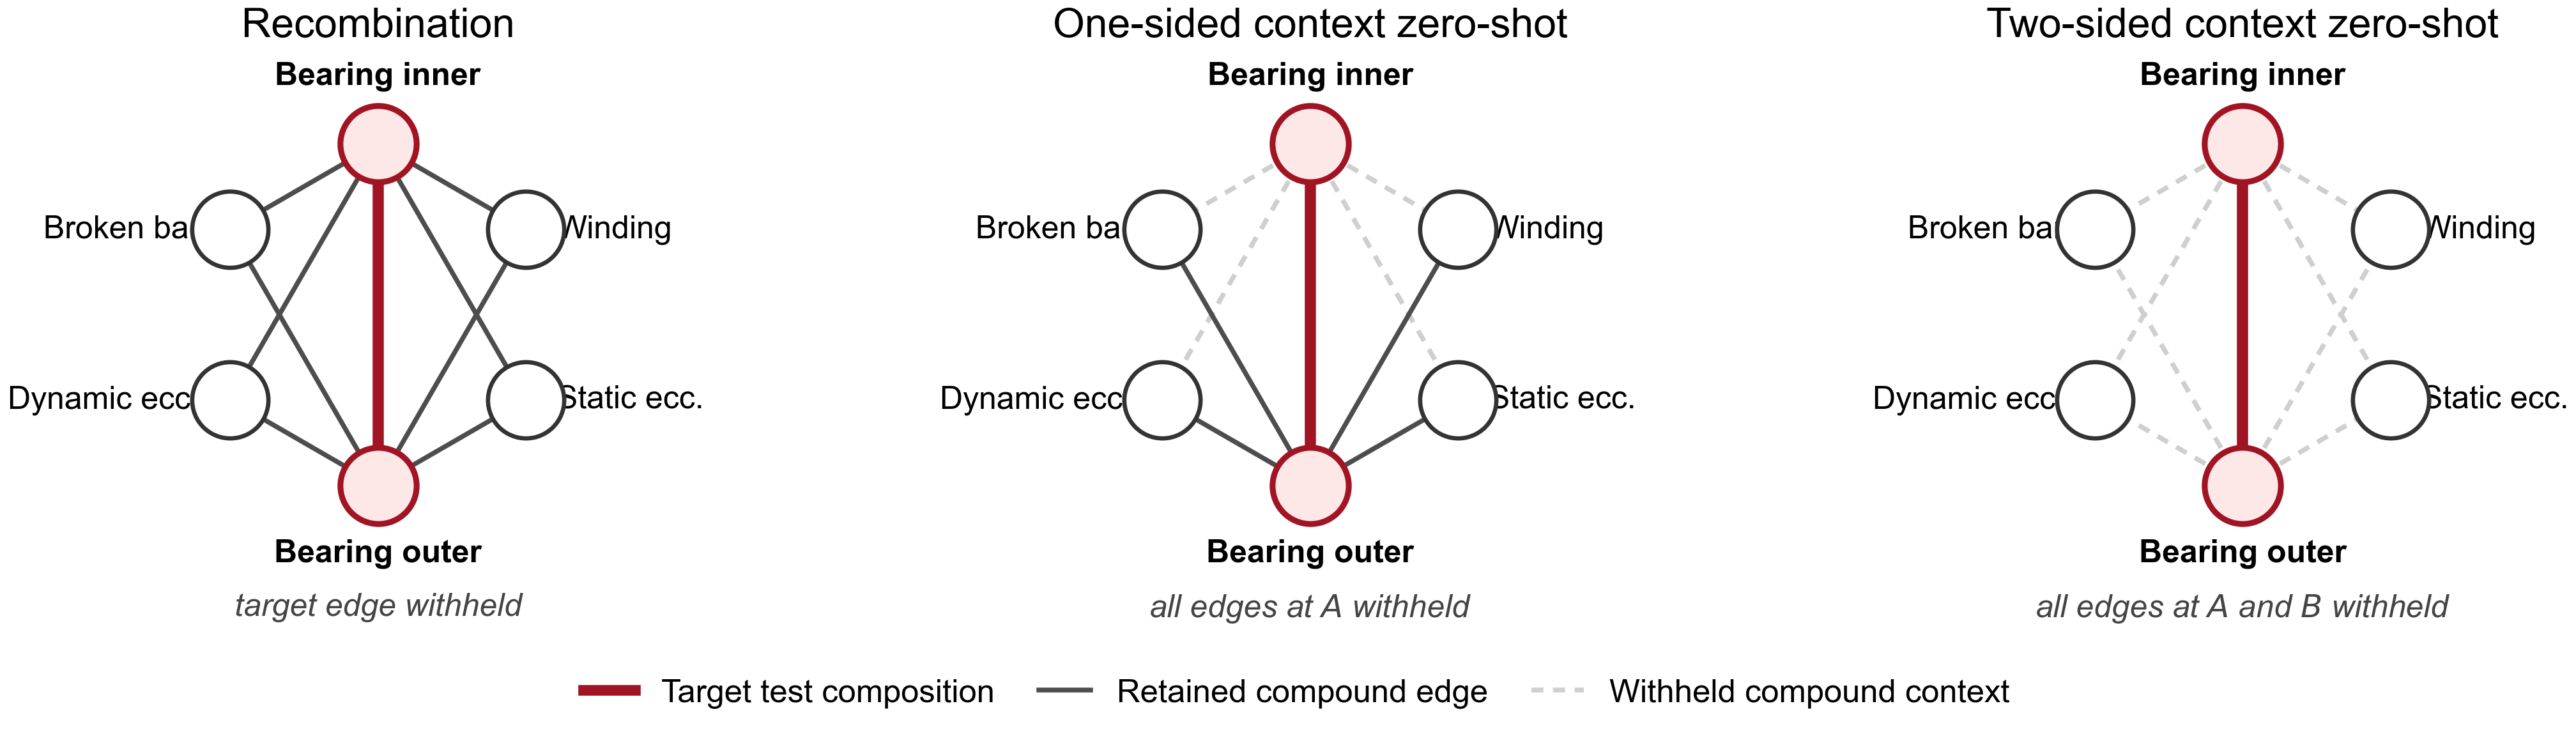
\includegraphics[width=\textwidth]{fig1_regimes}
\caption{Graph interpretation of the three compound-context evaluation
regimes. Nodes denote fault mechanisms participating in the compound
subgraph, edges denote observed compound compositions, and the red edge
denotes the target test composition. Recombination withholds only the
target edge; one-sided context zero-shot removes all compound-context
exposure for one target constituent; and two-sided context zero-shot
removes compound exposure for both target constituents.}
\label{fig:regimes}
\end{figure*}

Let the target test composition be
\begin{equation}
\mathcal{C}^{*} = \{A, B\}.
\end{equation}
Three levels of compound-context exposure were considered.

\subsubsection{Recombination}
The exact pair $A{+}B$ was excluded from training, while both $A$ and $B$
remained observable in other compound compositions. If
$d_{\mathrm{cmp}}(f)$ denotes the number of distinct compound contexts
containing constituent $f$ in the outer training set, the recombination
regime satisfies
\begin{equation}
d_{\mathrm{cmp}}(A) > 0, \qquad d_{\mathrm{cmp}}(B) > 0.
\end{equation}
Thus, the constituent mechanisms were familiar in compound operation, but
their particular edge or pairing was novel.

\subsubsection{One-Sided Compound-Context Zero-Shot}
In this regime, one constituent was completely removed from all compound
contexts while remaining available as a single fault. Without loss of
generality,
\begin{equation}
d_{\mathrm{cmp}}(A) = 0, \qquad d_{\mathrm{cmp}}(B) > 0.
\end{equation}
Both directional cases, $A$-unseen and $B$-unseen, were evaluated
separately.

\subsubsection{Two-Sided Compound-Context Zero-Shot}
The most restrictive context regime removed all compound examples
containing either constituent,
\begin{equation}
d_{\mathrm{cmp}}(A) = 0, \qquad d_{\mathrm{cmp}}(B) = 0,
\end{equation}
while preserving their eligible single-fault examples. Consequently,
neither constituent had been observed in any compound context before
testing on $A{+}B$.

Each composition-context regime was further crossed with operating-condition
exposure. Let $c_i$ denote the operating-condition identifier of run $i$.
For the seen-condition setting,
\begin{equation}
c_{\mathrm{test}} \in \mathcal{C}_{\mathrm{train}},
\end{equation}
whereas for the unseen-condition setting,
\begin{equation}
c_{\mathrm{test}} \notin \mathcal{C}_{\mathrm{train}}.
\end{equation}
The complete experimental design therefore consisted of
\begin{equation}
3 \ \text{compound-context regimes} \times 2 \ \text{condition regimes},
\end{equation}
resulting in six principal evaluation scenarios.

All splitting was performed at the experimental-run level before any
classifier fitting. Composition identities were defined from the
constituent vector rather than severity-specific class names, thereby
preventing severity variants of the same constituent combination from
unintentionally leaking across the composition boundary. Because either
member of a target compound could be deprived of prior compound-context
exposure, the one-sided regime was evaluated in both directions.
Consequently, this regime produced 216 prediction rows from 108 unique
physical compound runs, whereas the recombination and two-sided regimes
each produced 108 prediction rows from 108 unique runs. The two directional
predictions associated with the same physical run were never treated as
independent experimental units in uncertainty estimation; all bootstrap
analyses were clustered by physical run.

\subsection{Evaluation Metrics}
\label{sec:metrics}

Performance was evaluated using metrics that directly quantify recovery of
the constituent set rather than only conventional sample-level
classification. The overall constituent recall was defined as
\begin{equation}
R_{\mathrm{const}} =
\frac{\sum_{i=1}^{N}\sum_{k=1}^{K} y_{i,k}\hat{y}_{i,k}}
     {\sum_{i=1}^{N}\sum_{k=1}^{K} y_{i,k}}.
\end{equation}
Exact constituent-set recovery was computed as
\begin{equation}
\mathrm{EM} = \frac{1}{N}\sum_{i=1}^{N}
\mathbb{I}\left(\hat{\mathbf{y}}_i = \mathbf{y}_i\right).
\end{equation}
The average number of incorrectly added mechanisms per prediction row was
\begin{equation}
\mathrm{FA} = \frac{1}{N}\sum_{i=1}^{N}\sum_{k=1}^{K}
\left(1 - y_{i,k}\right)\hat{y}_{i,k}.
\end{equation}
The fraction of compound predictions for which at least one true
constituent was recovered was
\begin{equation}
R_{\mathrm{any}} = \frac{1}{N}\sum_{i=1}^{N}
\mathbb{I}\left(\sum_{k=1}^{K} y_{i,k}\hat{y}_{i,k} > 0\right),
\end{equation}
whereas recovery of all true constituents, irrespective of additional false
activations, was defined as
\begin{equation}
R_{\mathrm{all}} = \frac{1}{N}\sum_{i=1}^{N}
\mathbb{I}\left(\sum_{k=1}^{K} y_{i,k}\hat{y}_{i,k}
= \sum_{k=1}^{K} y_{i,k}\right).
\end{equation}
Micro-averaged $F_1$ was calculated over all constituent decisions as
\begin{equation}
\Fmicro = \frac{2TP}{2TP + FP + FN}.
\end{equation}
Because some evaluation subsets contained only a subset of the nine
constituents, macro-$F_1$ was additionally calculated over active
constituents,
\begin{equation}
\Factive = \frac{1}{|\mathcal{K}_{+}|}
\sum_{k \in \mathcal{K}_{+}} F_{1,k},
\end{equation}
where $\mathcal{K}_{+}$ denotes the constituents having at least one
positive test instance.

\subsection{Within-Pair Detectability and Cross-Partner Transfer}
\label{sec:transfer}

To determine whether poor constituent recovery reflected an absence of
measurable evidence, an oracle detectability analysis was performed. For
constituent $A$ in target compound $A{+}B$, the compound state was compared
directly with the corresponding single-$B$ state,
\begin{equation}
A{+}B \quad \text{vs.} \quad B.
\end{equation}
The resulting within-pair discriminability was quantified using ROC AUC and
denoted $\mathrm{AUC}^{\mathrm{within}}_{A|B}$.

A stronger transfer analysis evaluated whether evidence for $A$ learned
from eligible compound contexts other than the target composition remained
useful when $A$ occurred with partner $B$. The target pair $A{+}B$ was
excluded from training and the resulting fixed-orientation score was
evaluated on $A{+}B$ vs.\ $B$. The conventional directional cross-partner
AUC was denoted $\mathrm{AUC}^{A|B}_{\mathrm{dir}}$.

Because an AUC below 0.5 can reflect reversed ranking rather than absence
of separability, an orientation-free diagnostic measure was additionally
defined as
\begin{equation}
\mathrm{AUC}_{\mathrm{sep}} =
\max\left(\mathrm{AUC}_{\mathrm{dir}}, 1 - \mathrm{AUC}_{\mathrm{dir}}\right)
= 0.5 + \left|\mathrm{AUC}_{\mathrm{dir}} - 0.5\right|.
\label{eq:aucsep}
\end{equation}
$\mathrm{AUC}_{\mathrm{sep}}$ was used only to characterize rank
separability and was not interpreted as deployable classification
performance, because post-hoc inversion of an unknown target score would
require target-label information. The fixed-orientation transfer gap was
defined as
\begin{equation}
\Delta_{\mathrm{transfer}} =
\mathrm{AUC}^{\mathrm{within}}_{A|B} - \mathrm{AUC}^{A|B}_{\mathrm{dir}}.
\end{equation}
This quantity characterizes degradation of the learned score orientation
and should not be interpreted directly as loss of orientation-free
separability.

Because the released recordings were acquired across multiple recording
dates, an additional recording-sensitivity analysis was performed.
Acquisition timestamps were recovered from the original file names for 287
of the 288 runs, spanning seven recording dates. The only duplicated
fault--condition state available in two distinct recordings was used as a
nuisance-control experiment. In addition, compound pairs acquired on the
same date and sharing one constituent were compared under matched operating
conditions to reduce recording-date mismatch in the interpretation of
within-pair separability. These analyses were treated as sensitivity
controls rather than as causal estimates of acquisition-session effects.

\subsection{Physical-Signature Preservation Analysis}
\label{sec:preservation}

A complementary feature-level analysis characterized how predefined
physical signatures changed when a constituent was embedded in a compound
fault. Only the mechanism-specific curated feature families defined
independently of the cross-partner results were used. For feature $j$
associated with constituent $A$, let $\delta_j^{A}$ denote its signed
standardized evidence under the single-fault reference and
$\delta_j^{A|B}$ denote the evidence for the same feature when $A$ occurred
together with partner $B$. Feature preservation was summarized as
\begin{equation}
\rho_j^{A|B} = \frac{\delta_j^{A|B}}{\delta_j^{A}}.
\label{eq:preservation}
\end{equation}
Negative values indicate feature-level sign reversal, values between zero
and one indicate suppression, values around one indicate approximate
preservation, and values greater than one indicate amplification. This
analysis was used to characterize heterogeneity of predefined physical
signatures and was not interpreted as a causal decomposition of the
multivariate classifier score.

\subsection{Statistical Analysis}
\label{sec:stats}

Uncertainty of the principal constituent-level metrics was estimated using
nonparametric cluster bootstrap resampling at the physical-run level. In
the one-sided regime, both directional predictions associated with a
physical run were retained within the same bootstrap cluster. In addition
to protocol-specific confidence intervals, paired bootstrap contrasts were
computed because the same physical compound runs contributed to the
compared context regimes. Three prespecified contrasts were evaluated
separately under seen and unseen operating conditions:
\begin{align}
\Delta_{R-O} &= M_{\mathrm{recomb}} - M_{\mathrm{one}},\\
\Delta_{R-T} &= M_{\mathrm{recomb}} - M_{\mathrm{two}},\\
\Delta_{O-T} &= M_{\mathrm{one}} - M_{\mathrm{two}},
\end{align}
where $M$ denotes the metric of interest. The 95\% confidence interval was
obtained from the 2.5th and 97.5th percentiles of the paired bootstrap
distribution. A contrast was considered resolved when this interval
excluded zero. To formally test whether the effect of compound-context
deprivation changed under operating-condition shift, a
difference-of-differences statistic was also evaluated,
\begin{equation}
\Delta_{\mathrm{int}} = \Delta_{\mathrm{unseen}} - \Delta_{\mathrm{seen}},
\label{eq:interaction}
\end{equation}
where $\Delta$ denotes the paired difference between recombination and the
corresponding context-zero-shot regime. Confidence intervals were estimated
using 5000 paired cluster-bootstrap resamples at the physical-run level.
For the auxiliary closed-set experiment, 95\% confidence intervals were
estimated using 5000 stratified run-level bootstrap resamples within the
original 24 diagnostic classes.

For cross-partner transfer, evidence for reversed score orientation was
tested using
\begin{equation}
T = \left|\mathrm{AUC}_{\mathrm{dir}} - 0.5\right|.
\label{eq:polarity}
\end{equation}
Positive and negative scores were exchanged within matched operating
conditions under permutation, thereby preserving the paired experimental
structure. Family-wise multiplicity across the 18 directed
constituent--partner relations was controlled using the Holm procedure. A
relation was described as a statistically supported polarity reversal only
when its directional AUC was below 0.5, its bootstrap interval remained
below 0.5, and the Holm-adjusted permutation analysis supported departure
from chance orientation.

\section{Results}
\label{sec:results}

\subsection{Closed-Set Discrimination and the Generalization Gap}
\label{sec:closedsetresults}

Before evaluating compositional generalization, an auxiliary closed-set
experiment was conducted to determine whether the dataset was intrinsically
difficult to discriminate when all diagnostic classes were represented
during training. The 24-class closed-set classifier achieved an accuracy of
0.9132, a balanced accuracy of 0.9134, and a macro-$F_1$ score of 0.9119,
as summarized in Table~\ref{tab:closedset}.

\begin{table}[!t]
\caption{Closed-set multiclass diagnostic performance with 95\% bootstrap
confidence intervals.}
\label{tab:closedset}
\centering
\begin{tabular}{l c c}
\toprule
Metric & Estimate & 95\% CI \\
\midrule
Accuracy          & 0.9132 & $[0.8854, 0.9375]$ \\
Balanced accuracy & 0.9134 & $[0.8856, 0.9377]$ \\
Macro-$F_1$       & 0.9119 & $[0.8826, 0.9366]$ \\
\bottomrule
\end{tabular}
\end{table}

These results demonstrate strong conventional closed-set discriminability
when all diagnostic classes are represented during training. Consequently,
the substantially lower constituent-level performance observed under the
crossed protocols is unlikely to arise solely from poor baseline
separability; rather, it emerges under the additional requirements of
composition, compound-context, and operating-condition generalization.

\subsection{Crossed Composition--Context--Condition Generalization}
\label{sec:crossedresults}

The proposed crossed evaluation protocol was applied to all 108 unique
physical compound-fault runs. Each target compound was evaluated under
recombination, one-sided compound-context zero-shot, and two-sided
compound-context zero-shot regimes, with each regime further separated into
seen- and unseen-operating-condition settings. In the one-sided regime,
both directional removals were evaluated because either constituent could
be the mechanism deprived of compound-context exposure.
Table~\ref{tab:crossed} summarizes the principal constituent-level results.

\begin{table*}[!t]
\caption{Constituent-level generalization performance under crossed
composition-context and operating-condition regimes. EM denotes exact
constituent-set recovery, $R_{\mathrm{const}}$ denotes constituent recall,
FA/run denotes the mean number of incorrectly added inactive constituents
per compound prediction row, and $R_{\mathrm{any}}$ and $R_{\mathrm{all}}$
denote recovery of at least one and all true constituents, respectively.}
\label{tab:crossed}
\centering
\begin{tabular}{l l c c c c c c c}
\toprule
Condition & Context regime & Active Macro-$F_1$ & Micro-$F_1$ & EM &
$R_{\mathrm{const}}$ & FA/run & $R_{\mathrm{any}}$ & $R_{\mathrm{all}}$ \\
\midrule
Seen   & One-sided     & 0.5890 & 0.6581 & 0.1204 & 0.6505 & 0.6528 & 0.9259 & 0.3750 \\
Seen   & Recombination & 0.6177 & 0.6775 & 0.1389 & 0.6759 & 0.6389 & 0.9352 & 0.4167 \\
Seen   & Two-sided     & 0.5994 & 0.6620 & 0.1111 & 0.6620 & 0.6759 & 0.9444 & 0.3796 \\
Unseen & One-sided     & 0.5761 & 0.6452 & 0.1111 & 0.6481 & 0.7222 & 0.9398 & 0.3565 \\
Unseen & Recombination & 0.6177 & 0.6865 & 0.1574 & 0.6944 & 0.6574 & 0.9444 & 0.4444 \\
Unseen & Two-sided     & 0.5588 & 0.6311 & 0.0833 & 0.6296 & 0.7315 & 0.9352 & 0.3241 \\
\bottomrule
\end{tabular}
\end{table*}

\begin{table*}[!t]
\caption{Input-independent constant-predictor references on the 108
compound runs. These references quantify performance obtainable from
constituent prevalence alone.}
\label{tab:trivial}
\centering
\begin{tabular}{l c c c c c c}
\toprule
Constant prediction & Micro-$F_1$ & EM & $R_{\mathrm{const}}$ & FA/run &
$R_{\mathrm{any}}$ & $R_{\mathrm{all}}$ \\
\midrule
Inner $+$ outer                & 0.5556 & 0.1111 & 0.5556 & 0.8889 & 1.0000 & 0.1111 \\
Inner $+$ outer $+$ broken bar & 0.5333 & 0.0000 & 0.6667 & 1.6667 & 1.0000 & 0.3333 \\
Inner only                     & 0.3704 & 0.0000 & 0.2778 & 0.4444 & 0.5556 & 0.0000 \\
\bottomrule
\end{tabular}
\end{table*}

When both constituents retained prior exposure to other compound contexts,
previously unseen pairings remained partially recoverable. Under the
recombination protocol, micro-$F_1$ was 0.6775 under seen operating
conditions and 0.6865 when the operating condition was also unseen.
Constituent recall showed a similar pattern, reaching 0.6759 and 0.6944,
respectively.

Exact constituent-set recovery remained limited, ranging from 0.0833 to
0.1574 across the six crossed regimes. However, the trivial references in
Table~\ref{tab:trivial} show that some apparently favorable
partial-recovery metrics are strongly influenced by constituent prevalence.
In particular, the constant inner-plus-outer predictor achieves
$R_{\mathrm{any}} = 1.0$ without using the input signals. Consequently,
$R_{\mathrm{any}}$ is retained only as a descriptive measure and is not
interpreted as evidence of diagnostic skill.

Constituent recall alone is not sufficient to establish diagnostic skill in
this setting. The constant inner-plus-outer-plus-broken-bar predictor
reaches $R_{\mathrm{const}} = 0.6667$ without using the input signals, but
does so at the cost of 1.6667 false additions per run and zero exact
matches. Accordingly, constituent recall is interpreted jointly with false
additions, micro-$F_1$, and exact-set recovery throughout the remainder of
the analysis.

The locked logistic-regression detector achieved micro-$F_1$ values of
0.631--0.686 across the six crossed regimes, exceeding the best
constant-predictor micro-$F_1$ of 0.556. At the same time, FA/run remained
between 0.639 and 0.732, substantially below the 1.667 false additions
produced by the three-constituent constant reference and also below the
0.889 value of the constant inner-plus-outer predictor. Under
recombination, $R_{\mathrm{all}}$ reached 0.4167 and 0.4444 for seen and
unseen conditions, respectively, compared with 0.1111 for the
two-constituent constant reference. These results indicate nontrivial
constituent discrimination beyond prevalence-driven constant prediction,
while the low exact-match rates show that reliable exact decomposition of
unseen compound faults remains unresolved.

\subsection{Paired Effects of Compound-Context Deprivation}
\label{sec:pairedeffects}

Paired run-cluster bootstrap analysis was used to determine which
differences between the context regimes were supported beyond variation
across physical runs. Figure~\ref{fig:contrasts} summarizes the
prespecified contrasts for constituent recall and micro-$F_1$.

\begin{figure*}[!t]
\centering
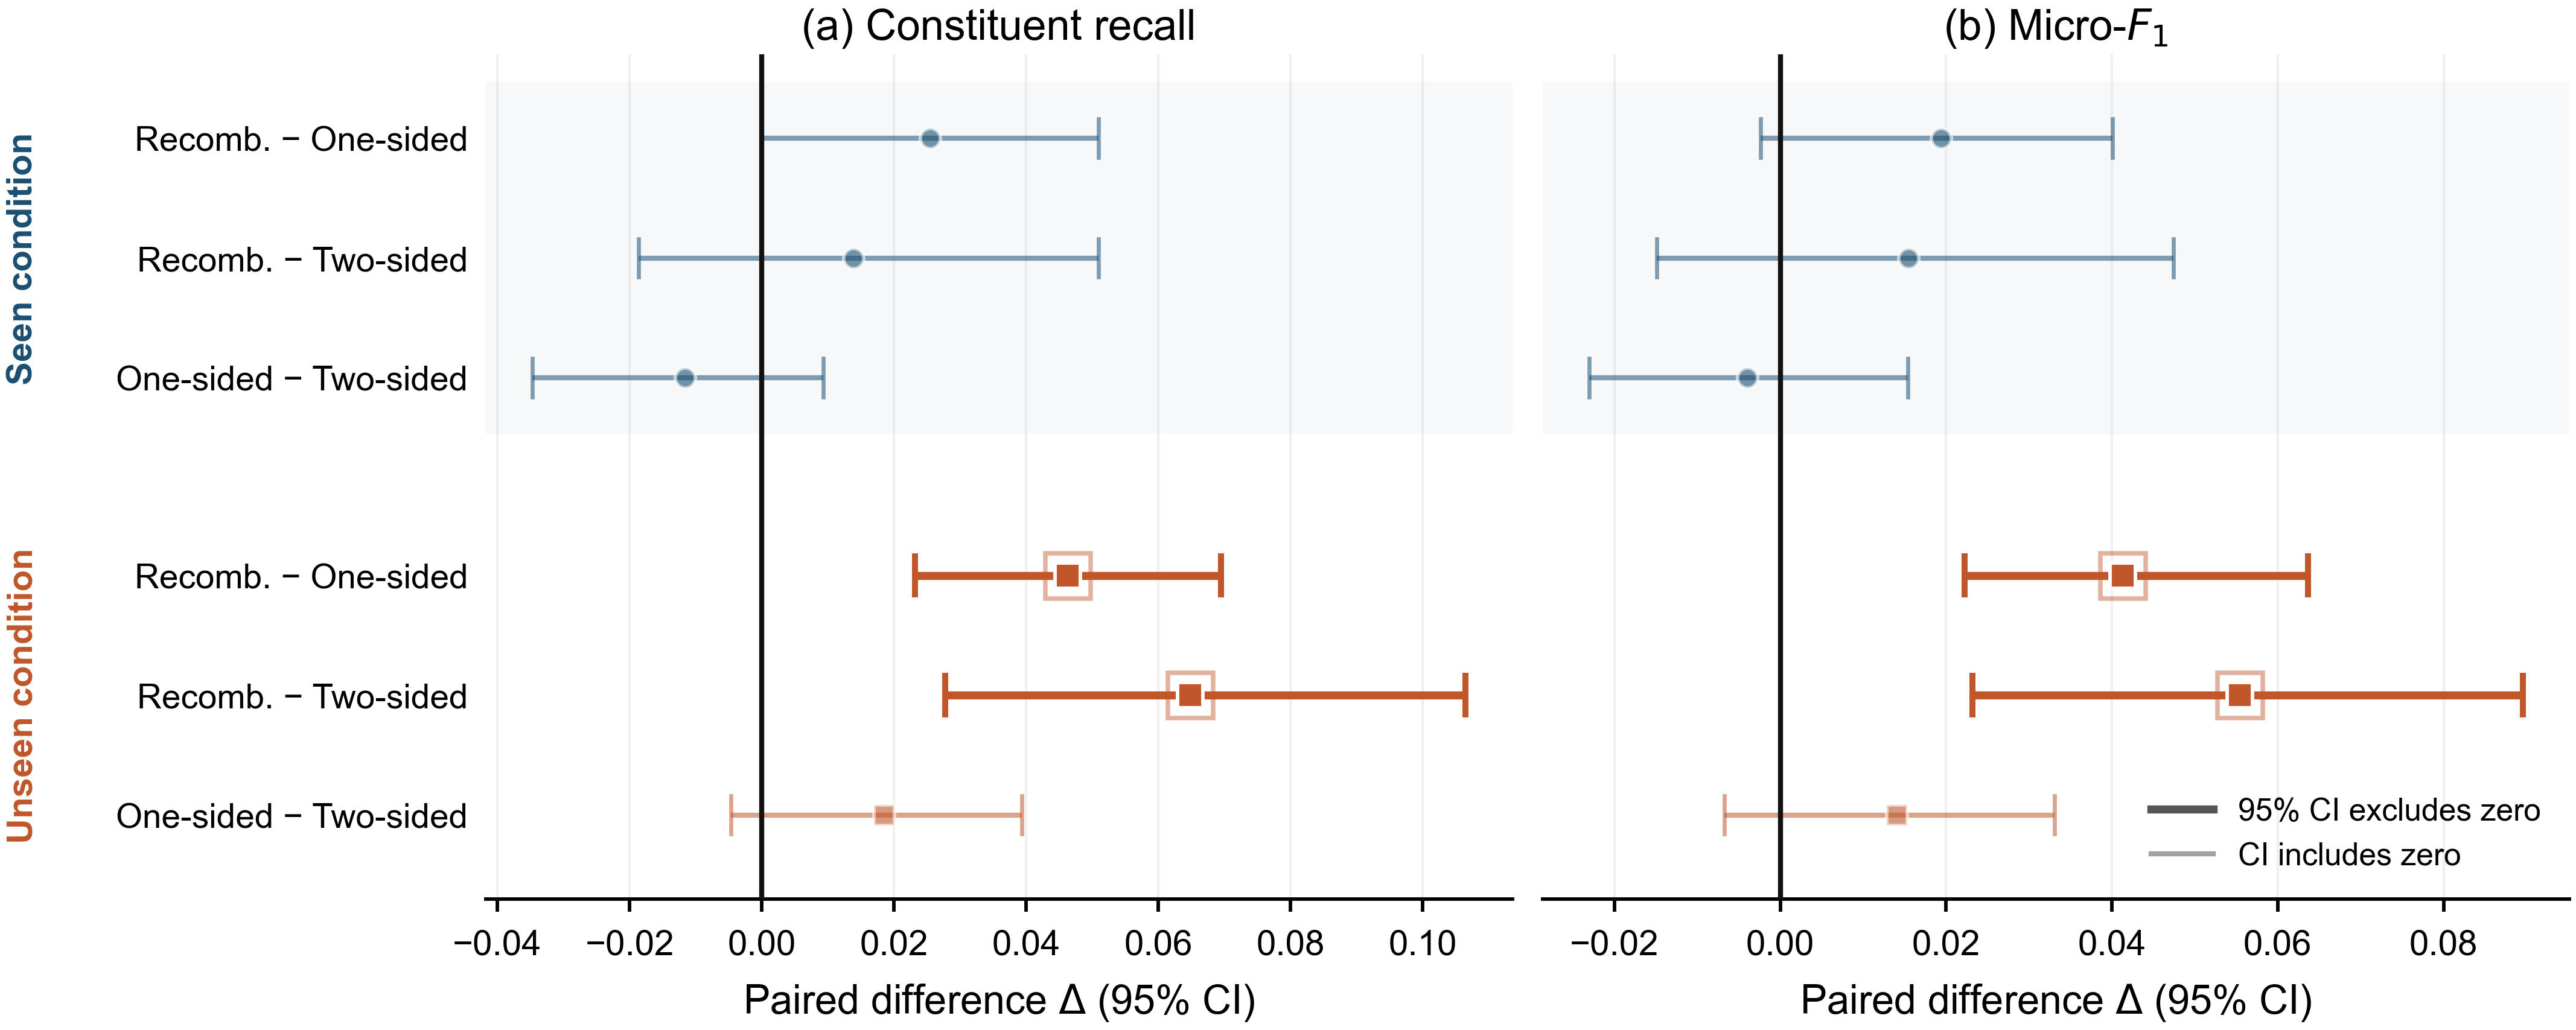
\includegraphics[width=\textwidth]{fig2_contrasts}
\caption{Paired run-cluster bootstrap differences between
composition-context regimes. Points denote paired differences in
constituent recall and micro-$F_1$, and horizontal bars denote 95\%
bootstrap confidence intervals. Positive values favor the first regime in
each contrast.}
\label{fig:contrasts}
\end{figure*}

Under seen operating conditions, the differences between recombination and
the context-zero-shot regimes were limited. For constituent recall, the
recombination--one-sided contrast was 0.0255 with a 95\% CI of
$[0.0000, 0.0509]$, whereas the recombination--two-sided contrast was
0.0139 with a 95\% CI of $[-0.0186, 0.0509]$. The corresponding
micro-$F_1$ contrasts also included zero.

A different pattern was observed when the target operating condition was
withheld. Relative to one-sided context zero-shot, recombination improved
constituent recall by 0.0463 (95\% CI: $[0.0231, 0.0694]$) and micro-$F_1$
by 0.0413 (95\% CI: $[0.0223, 0.0636]$). Relative to two-sided context
zero-shot, the recombination advantage was 0.0648 for constituent recall
(95\% CI: $[0.0278, 0.1065]$) and 0.0554 for micro-$F_1$ (95\% CI:
$[0.0232, 0.0895]$).

The one-sided--two-sided differences remained unresolved for both metrics
under unseen operating conditions. A formal difference-of-differences
analysis further showed that the penalty associated with complete
compound-context deprivation increased under operating-condition shift. For
recombination versus two-sided context zero-shot, the interaction
difference was 0.0400 for micro-$F_1$ (95\% CI: $[0.0088, 0.0731]$), 0.0509
for constituent recall (95\% CI: $[0.0185, 0.0880]$), and 0.0833 for
all-constituents recovery (95\% CI: $[0.0278, 0.1481]$). In contrast, the
recombination-versus-one-sided interaction was not resolved for
micro-$F_1$ or constituent recall, although the interaction for
all-constituents recovery was positive at 0.0463 (95\% CI:
$[0.0046, 0.1019]$). These findings indicate that operating-condition shift
amplifies the penalty of complete compound-context deprivation rather than
producing a uniform interaction across all context regimes.

Directional decomposition of the one-sided regime revealed substantial
mechanism dependence. When broken-bar compound context was withheld,
constituent recall remained high at 0.979 under seen conditions and 0.896
under unseen conditions. In contrast, withholding winding compound context
reduced recall to 0.438 and 0.479, respectively, while withholding
dynamic-eccentricity context yielded a recall of 0.500 under both condition
settings. Each of the 108 physical compound runs contributed exactly two
directional one-sided predictions, and all bootstrap uncertainty estimates
remained clustered by physical run.

\subsection{Sensitivity to Decision-Threshold Objective}
\label{sec:thresholdsensitivity}

The limited exact-match performance and non-negligible false-addition
counts motivated a post-hoc sensitivity analysis of the inner-CV threshold
objective. The original $F_1$-based thresholds were retained as the locked
primary analysis. Alternative $F_{0.5}$ and balanced-accuracy objectives
were evaluated only to characterize the precision--recall operating-point
trade-off and were not used for post-hoc model selection.

Precision-weighted $F_{0.5}$ calibration substantially reduced false
additions. Across the six crossed regimes, FA/run decreased from
0.639--0.731 under the locked $F_1$ thresholds to approximately
0.222--0.389, while exact-match recovery increased from 0.083--0.157 to
0.157--0.287. This gain was accompanied by lower constituent recall, which
decreased to approximately 0.583--0.644. Conversely, balanced-accuracy
thresholding increased constituent recall but also increased false
additions.

These results show that exact compound decomposition is strongly affected
by the operating point of the constituent detectors. Precision-oriented
thresholding suppresses over-diagnosis and improves exact-set recovery,
whereas recall-oriented thresholding recovers more true constituents at the
cost of additional constituent activations. As shown by the
classifier-family robustness analysis below, absolute decomposition quality
is also model-dependent. Consequently, the low exact-match performance of
the locked linear probe should not be interpreted as an intrinsic upper
bound imposed by the crossed protocol itself.

\subsection{Sensitivity to Single-Fault Severity Merging}
\label{sec:severityresults}

Removing low-severity single-fault support did not produce a uniform change
in constituent recall, exact-match recovery, or all-constituent recovery
across the crossed regimes. Most paired differences for these metrics had
95\% confidence intervals spanning zero, indicating that the principal
generalization findings were not driven by pooling low- and high-severity
single-fault examples.

The clearest differences were observed in false additions. Under seen
conditions, removing low-severity support increased FA/run from 0.653 to
0.755 in the one-sided regime ($\Delta = +0.102$, 95\% CI:
$[0.046, 0.162]$) and from 0.639 to 0.722 under recombination
($\Delta = +0.083$, 95\% CI: $[0.019, 0.157]$). Under unseen conditions,
the two-sided regime similarly increased from 0.731 to 0.843 FA/run
($\Delta = +0.111$, 95\% CI: $[0.037, 0.185]$). For seen-condition
recombination, micro-$F_1$ decreased from 0.677 to 0.651 when low-severity
support was removed ($\Delta = -0.026$, 95\% CI: $[-0.052, -0.002]$).
Other micro-$F_1$ differences were unresolved. Overall, the sensitivity
analysis indicates that severity merging does not account for the principal
crossed-generalization pattern and, in several regimes, the additional
low-severity support reduced over-diagnosis rather than artificially
inflating constituent recovery.

\subsection{Robustness Across Classifier Families}
\label{sec:familyresults}

The complete crossed protocol was additionally evaluated with
random-forest, RBF-SVM, and neural classifiers while retaining the same
constituent representation, curated feature families, outer evaluation
splits, and inner-CV threshold-calibration principles.
Table~\ref{tab:families} summarizes descriptive performance averaged across
the six crossed scenarios. The locked logistic-regression results remain
the primary analysis; the alternative classifiers are reported only as
robustness references.

\begin{table}[!t]
\caption{Descriptive classifier-family robustness averaged across the six
crossed evaluation scenarios. LR denotes logistic regression and MLP
denotes the three-hidden-layer feed-forward neural baseline.}
\label{tab:families}
\centering
\begin{tabular}{l c c c c}
\toprule
Model & Micro-$F_1$ & EM & $R_{\mathrm{const}}$ & FA/run \\
\midrule
LR      & 0.660 & 0.120 & 0.660 & 0.680 \\
RF      & 0.744 & 0.282 & 0.669 & 0.256 \\
RBF-SVM & 0.692 & 0.157 & 0.664 & 0.509 \\
MLP     & 0.737 & 0.310 & 0.659 & 0.256 \\
\bottomrule
\end{tabular}
\end{table}

Absolute decomposition performance was classifier dependent. Random forest
achieved the highest mean micro-$F_1$ (0.744), whereas the neural baseline
achieved the highest mean exact-match rate (0.310). Both random forest and
the neural baseline reduced mean FA/run to 0.256, compared with 0.680 for
the locked logistic-regression probe. In contrast, mean constituent recall
varied only from 0.659 to 0.669 across the four classifiers. Thus,
classifier family primarily affected the precision of constituent-set
formation and the number of additional activations rather than the overall
fraction of true constituents recovered.

The qualitative recombination advantage was nevertheless retained across
all four classifier families. Under unseen operating conditions, the
recombination--two-sided difference in micro-$F_1$ was 0.055 for logistic
regression, 0.051 for random forest, 0.032 for RBF-SVM, and 0.023 for the
neural baseline. The corresponding constituent-recall differences were
0.065, 0.065, 0.069, and 0.032, respectively. These descriptive results
indicate that the adverse effect of complete compound-context deprivation
is not unique to the locked linear classifier.

\subsection{Oracle Detectability and Cross-Partner Constituent Transfer}
\label{sec:oracleresults}

To determine whether unsuccessful constituent recovery resulted from the
physical disappearance of a fault signature, a within-pair oracle analysis
was first performed. For each directed compound relation $A|B$,
measurements from the compound state $A{+}B$ were compared with the
corresponding single-$B$ reference while retaining the same constituent of
interest $A$.

All 18 directed constituent--partner tests exhibited strong within-pair
discriminability. The condition-held-out within-pair AUC ranged from 0.9167
to 1.000, with a median of 1.000. Thus, the target compound and its
corresponding partner-only reference remained strongly separable in the
broader physics-feature space. However, the recording-sensitivity control
showed that the two available recordings of the same bearing-outer fault
under the same operating condition were themselves nearly perfectly
separable ($\mathrm{AUC} = 0.998$). High within-pair AUC therefore cannot
be attributed uniquely to the additional constituent and may partly reflect
recording-specific nuisance variation.

A complementary same-date control reduced recording-date mismatch. Eight
pairs of compound states acquired on the same date shared one constituent
and all 12 operating conditions, yielding 16 directed matched comparisons.
Leave-one-condition-out AUCs ranged from 0.972 to 1.000. In particular,
static eccentricity in the bearing-outer context remained perfectly
separable when the alternative same-date compound contained either broken
bar or winding with the same bearing-outer partner ($\mathrm{AUC} = 1.000$
in both comparisons). Because these reference compounds contain a different
non-target constituent, the controls do not causally isolate the target
mechanism; nevertheless, they show that the observed compound-state
discriminability cannot be explained solely by recording-date mismatch.

Accordingly, within-pair detectability does not establish that the same
evidence is transferable across compound partners. Cross-partner
experiments were therefore performed by learning constituent $A$ from other
compound contrasts, such as $A{+}C$ versus $C$, and evaluating the
resulting detector on $A{+}B$ versus $B$.

Under seen operating conditions, the primary cross-partner protocol
achieved a median AUC of 0.905 across the 18 directed tests, with a mean
AUC of 0.815. Thirteen of the 18 directed tests achieved an AUC of at least
0.80, and 15 achieved an AUC of at least 0.70. When the target operating
condition was also withheld, the median AUC remained high at 0.884 and the
mean AUC was 0.803.

These aggregate values indicate that constituent evidence is often
transferable across partners. Nevertheless, the transfer behavior was
highly heterogeneous. Selected examples are reported in
Table~\ref{tab:transfer}. The complete pattern of directional cross-partner
transfer is shown in Figure~\ref{fig:heatmap}.

\begin{table*}[!t]
\caption{Selected directed cross-partner transfer results. The within-pair
AUC measures detectability of constituent $A$ in the target pair, whereas
the cross-partner AUC measures transfer of evidence learned from other
compound partners.}
\label{tab:transfer}
\centering
\begin{tabular}{l l l c c c}
\toprule
Target composition & Constituent $A$ & Partner $B$ &
\makecell{Within-pair\\AUC} & \makecell{Cross-partner\\AUC (seen)} &
\makecell{Cross-partner\\AUC (unseen)} \\
\midrule
Bearing inner $+$ bearing outer        & Bearing outer        & Bearing inner        & 1.000 & 1.000 & 1.000 \\
Bearing inner $+$ dynamic eccentricity & Bearing inner        & Dynamic eccentricity & 1.000 & 0.944 & 0.931 \\
Bearing inner $+$ broken bar           & Broken bar           & Bearing inner        & 1.000 & 0.893 & 0.851 \\
Bearing inner $+$ dynamic eccentricity & Dynamic eccentricity & Bearing inner        & 1.000 & 0.711 & 0.653 \\
Bearing outer $+$ static eccentricity  & Static eccentricity  & Bearing outer        & 0.917 & 0.000 & 0.000 \\
Bearing outer $+$ winding              & Winding              & Bearing outer        & 0.917 & 0.333 & 0.340 \\
\bottomrule
\end{tabular}
\end{table*}

\begin{figure*}[!t]
\centering
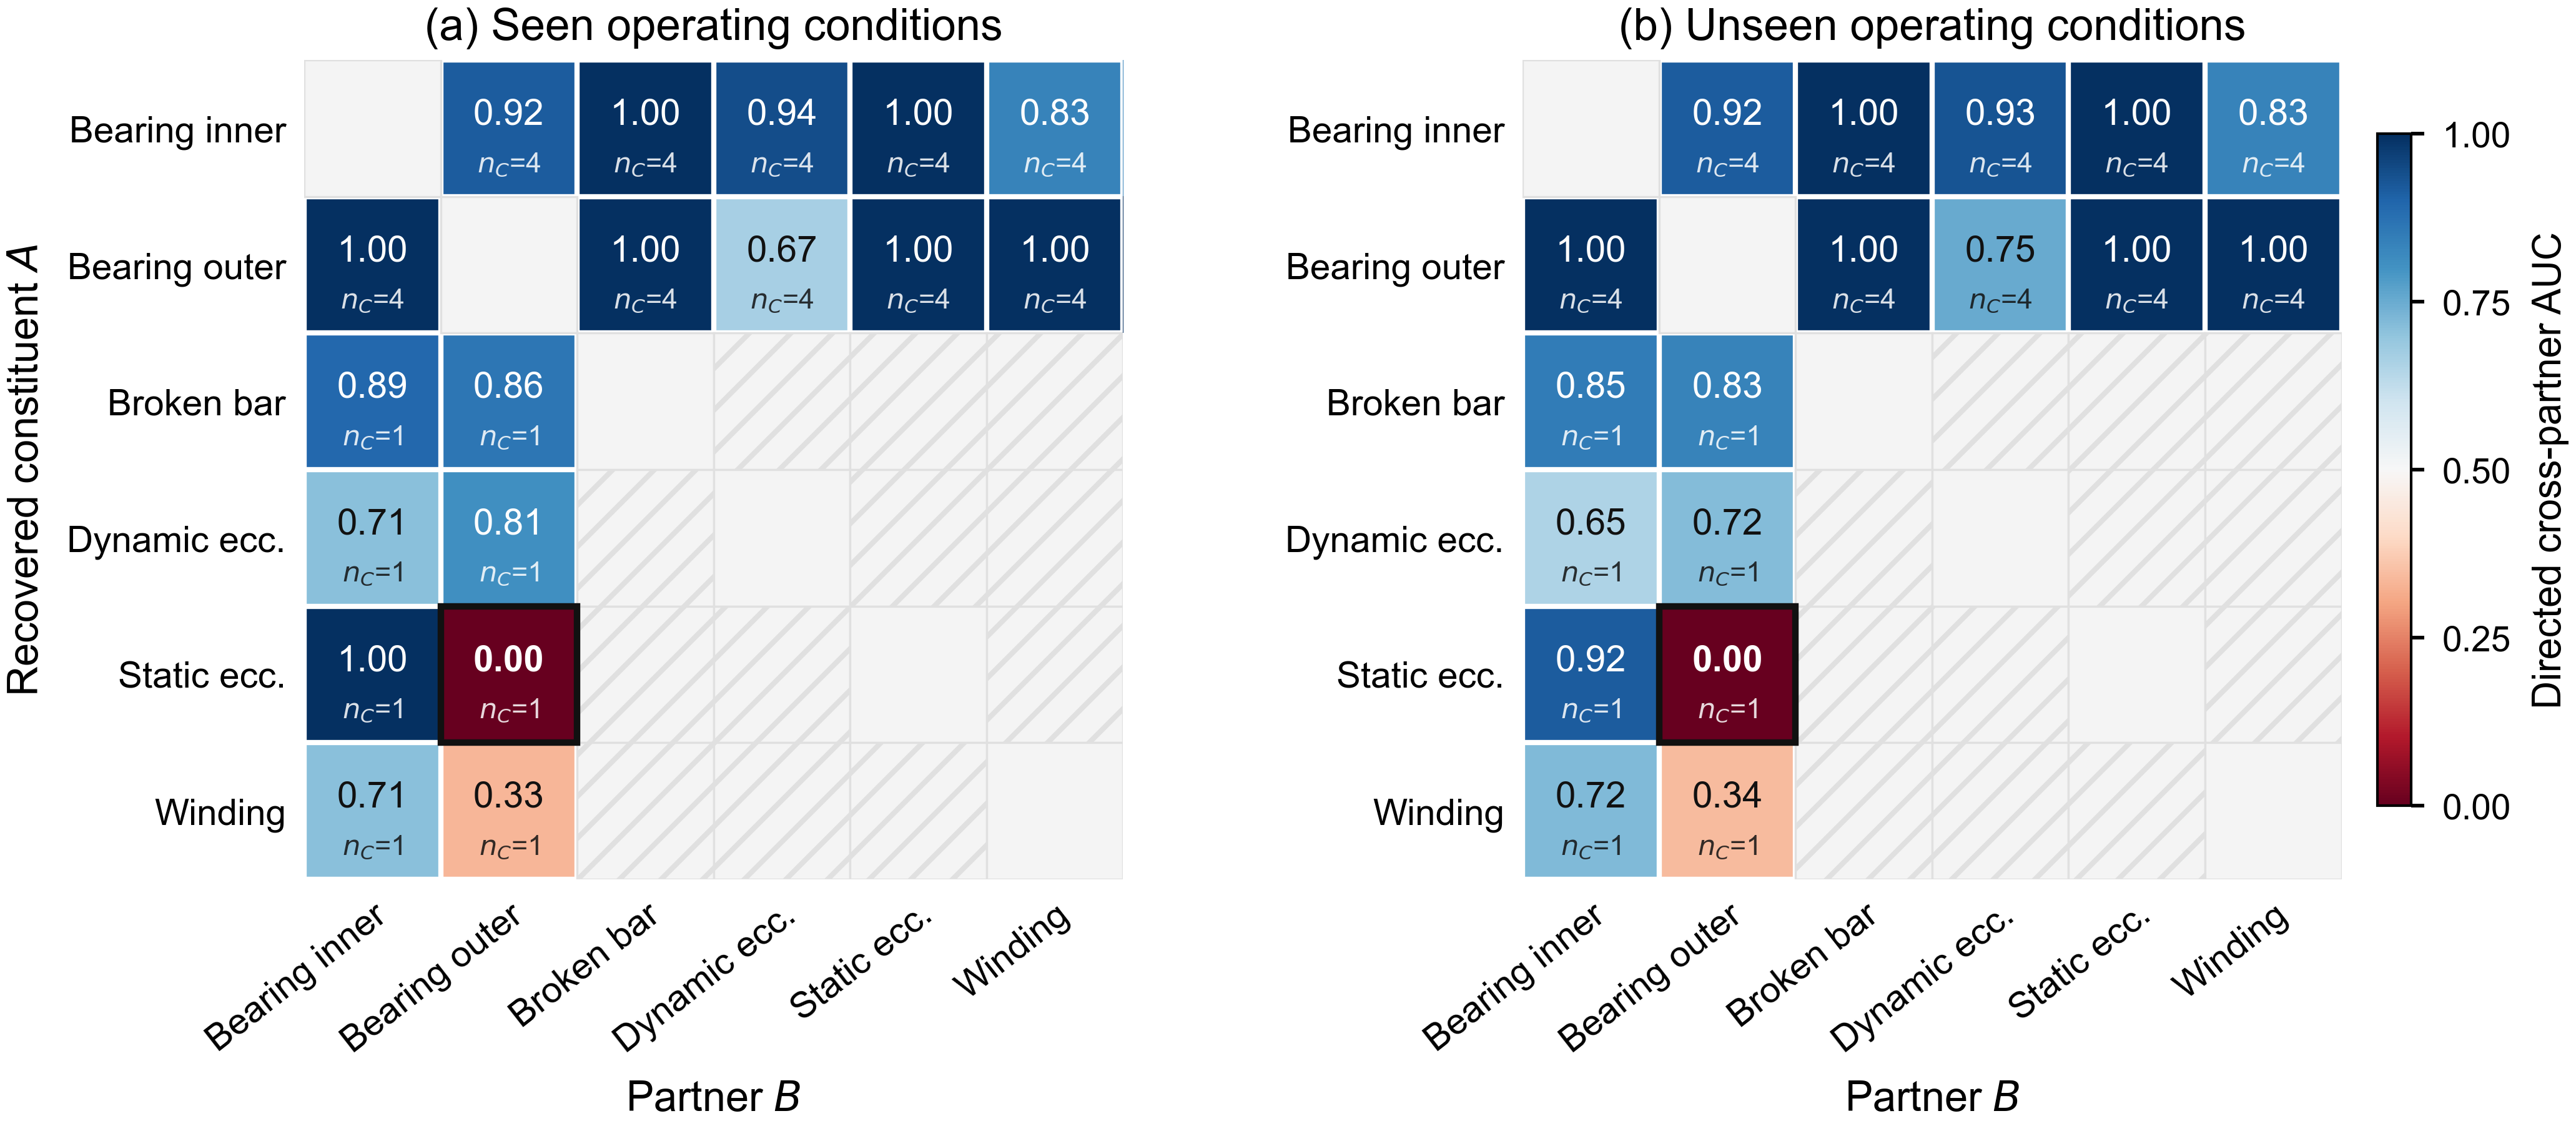
\includegraphics[width=\textwidth]{fig3_transfer_heatmap}
\caption{Directional cross-partner transfer AUC for the primary
other-partners transfer protocol. Rows denote the constituent $A$ to be
recovered and columns denote partner $B$ in the target compound. Values
below 0.5 indicate below-chance fixed-orientation ranking and do not by
themselves establish statistically supported polarity reversal. $n_C$
denotes the number of eligible compound training contexts available for the
recovered constituent.}
\label{fig:heatmap}
\end{figure*}

The contrast between within-pair and cross-partner performance was
particularly pronounced for static eccentricity in the presence of the
bearing-outer fault. Within the target pair, static eccentricity remained
strongly detectable, with $\mathrm{AUC}^{\mathrm{within}} = 0.9167$.
However, evidence learned from other eligible compound contexts produced a
fixed-orientation directional AUC of
\begin{equation}
\mathrm{AUC}_{\mathrm{dir}} = 0.000
\end{equation}
under both seen and unseen operating conditions. The corresponding
orientation-free separability was
\begin{equation}
\mathrm{AUC}_{\mathrm{sep}} = 1.000,
\end{equation}
indicating perfect rank separability in the opposite orientation. This was
the only directed constituent--partner relation classified as a
statistically supported score-orientation reversal after multiplicity
correction, with Holm-adjusted $p = 0.0136$ under seen conditions and
$p = 0.0108$ under unseen conditions. The statistical test establishes a
reproducible reversal of the fixed-score ordering, but it does not
establish that the reversal is caused exclusively by a physical inversion
of the static-eccentricity signature. Given the strong recording-identity
separability observed in the nuisance control, partner-dependent
constituent reorientation and acquisition-related variation remain
plausible, non-exclusive contributors to this result.

Winding in the bearing-outer composition also produced below-chance
directional AUCs of 0.3333 and 0.3403 under seen and unseen operating
conditions, respectively. However, its orientation-free separability was
only approximately 0.67 and the Holm-adjusted polarity tests were not
significant. This relation was therefore classified as
orientation-ambiguous rather than as a statistically supported
score-orientation reversal.

Taken together, the within-pair and recording-sensitivity controls show
that compound states can remain strongly discriminable while the
orientation of a score learned from other compound partners may fail to
transfer. Because recording-specific structure is also detectable in the
feature space, this phenomenon is interpreted as context-dependent score
transfer rather than as causal proof of physical constituent-signature
inversion. Figure~\ref{fig:withinvstransfer} directly contrasts within-pair
detectability with directional cross-partner transfer across the evaluated
constituent--partner relations.

\begin{figure}[!t]
\centering
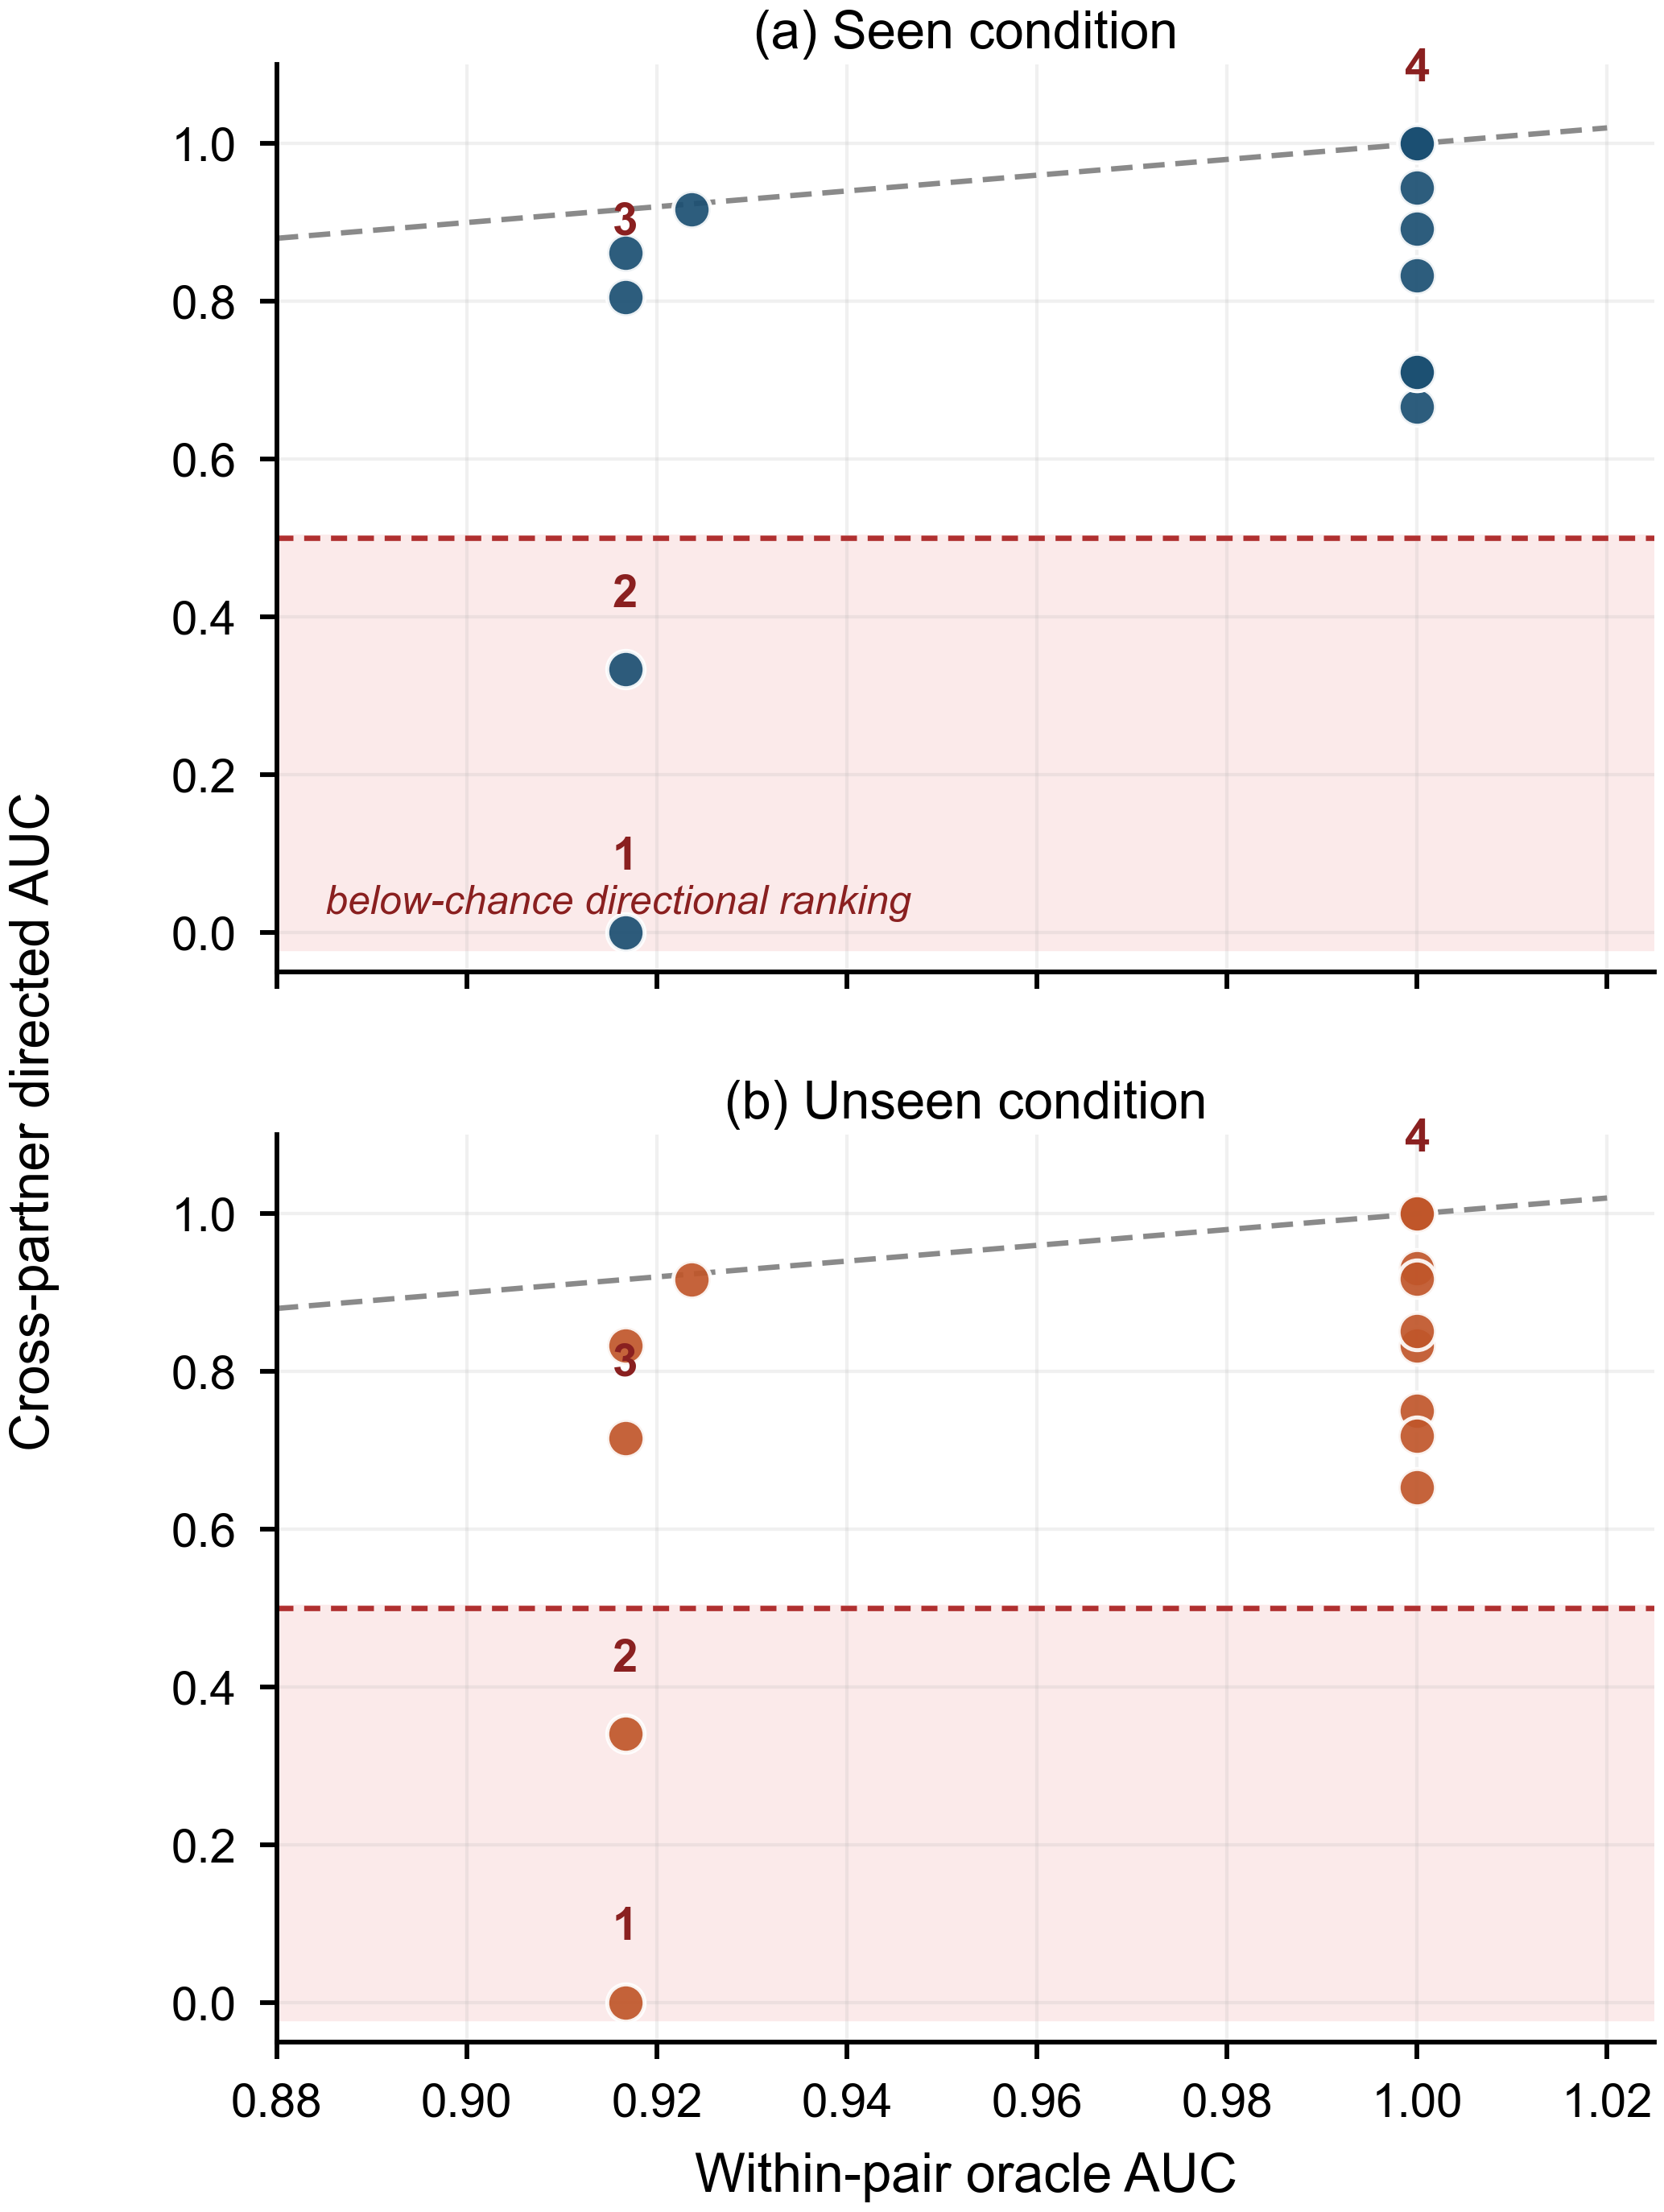
\includegraphics[width=\columnwidth]{fig4_withinpair_vs_transfer}
\caption{Within-pair oracle detectability versus directional cross-partner
transfer. The dashed horizontal line denotes chance-level directional
ranking. The shaded lower region represents below-chance directional
ranking; statistically supported polarity reversal requires the separate
polarity analysis described in Section~\ref{sec:stats}.}
\label{fig:withinvstransfer}
\end{figure}

\subsection{Physical-Signature Heterogeneity and Directional Failure
Modes}
\label{sec:heterogeneity}

Cross-partner transfer was strongly directional. For example, in the
bearing-outer plus static-eccentricity compound, evidence for bearing outer
transferred with an AUC of 1.000, whereas evidence for static eccentricity
in the opposite direction yielded a directional AUC of 0.000.
Transferability was therefore not a symmetric property of the compound
pair.

The feature-level preservation analysis further showed that multivariate
score-orientation reversal should not be equated with universal inversion
of the underlying physical descriptors. For static eccentricity in the
bearing-outer context, the median preservation ratio was 0.760, while
approximately 18.5\% of the eligible curated feature-condition observations
exhibited feature-level sign reversal and 31.4\% exhibited severe
suppression. Thus, most individual physical descriptors did not reverse
orientation even though the resulting multivariate cross-partner ranking
was completely inverted.

Conversely, strong feature suppression did not necessarily imply
score-orientation reversal. Bearing-outer evidence in the bearing-inner
compound showed a median preservation ratio of approximately 0.305 and a
severe-suppression rate of approximately 58\%, yet its cross-partner
directional AUC remained 1.000. Feature-level suppression and multivariate
score-orientation reversal therefore represent distinct forms of
partner-dependent behavior. Figure~\ref{fig:preservation} illustrates this
feature-level heterogeneity for static eccentricity under the two
bearing-partner contexts.

\begin{figure}[!t]
\centering
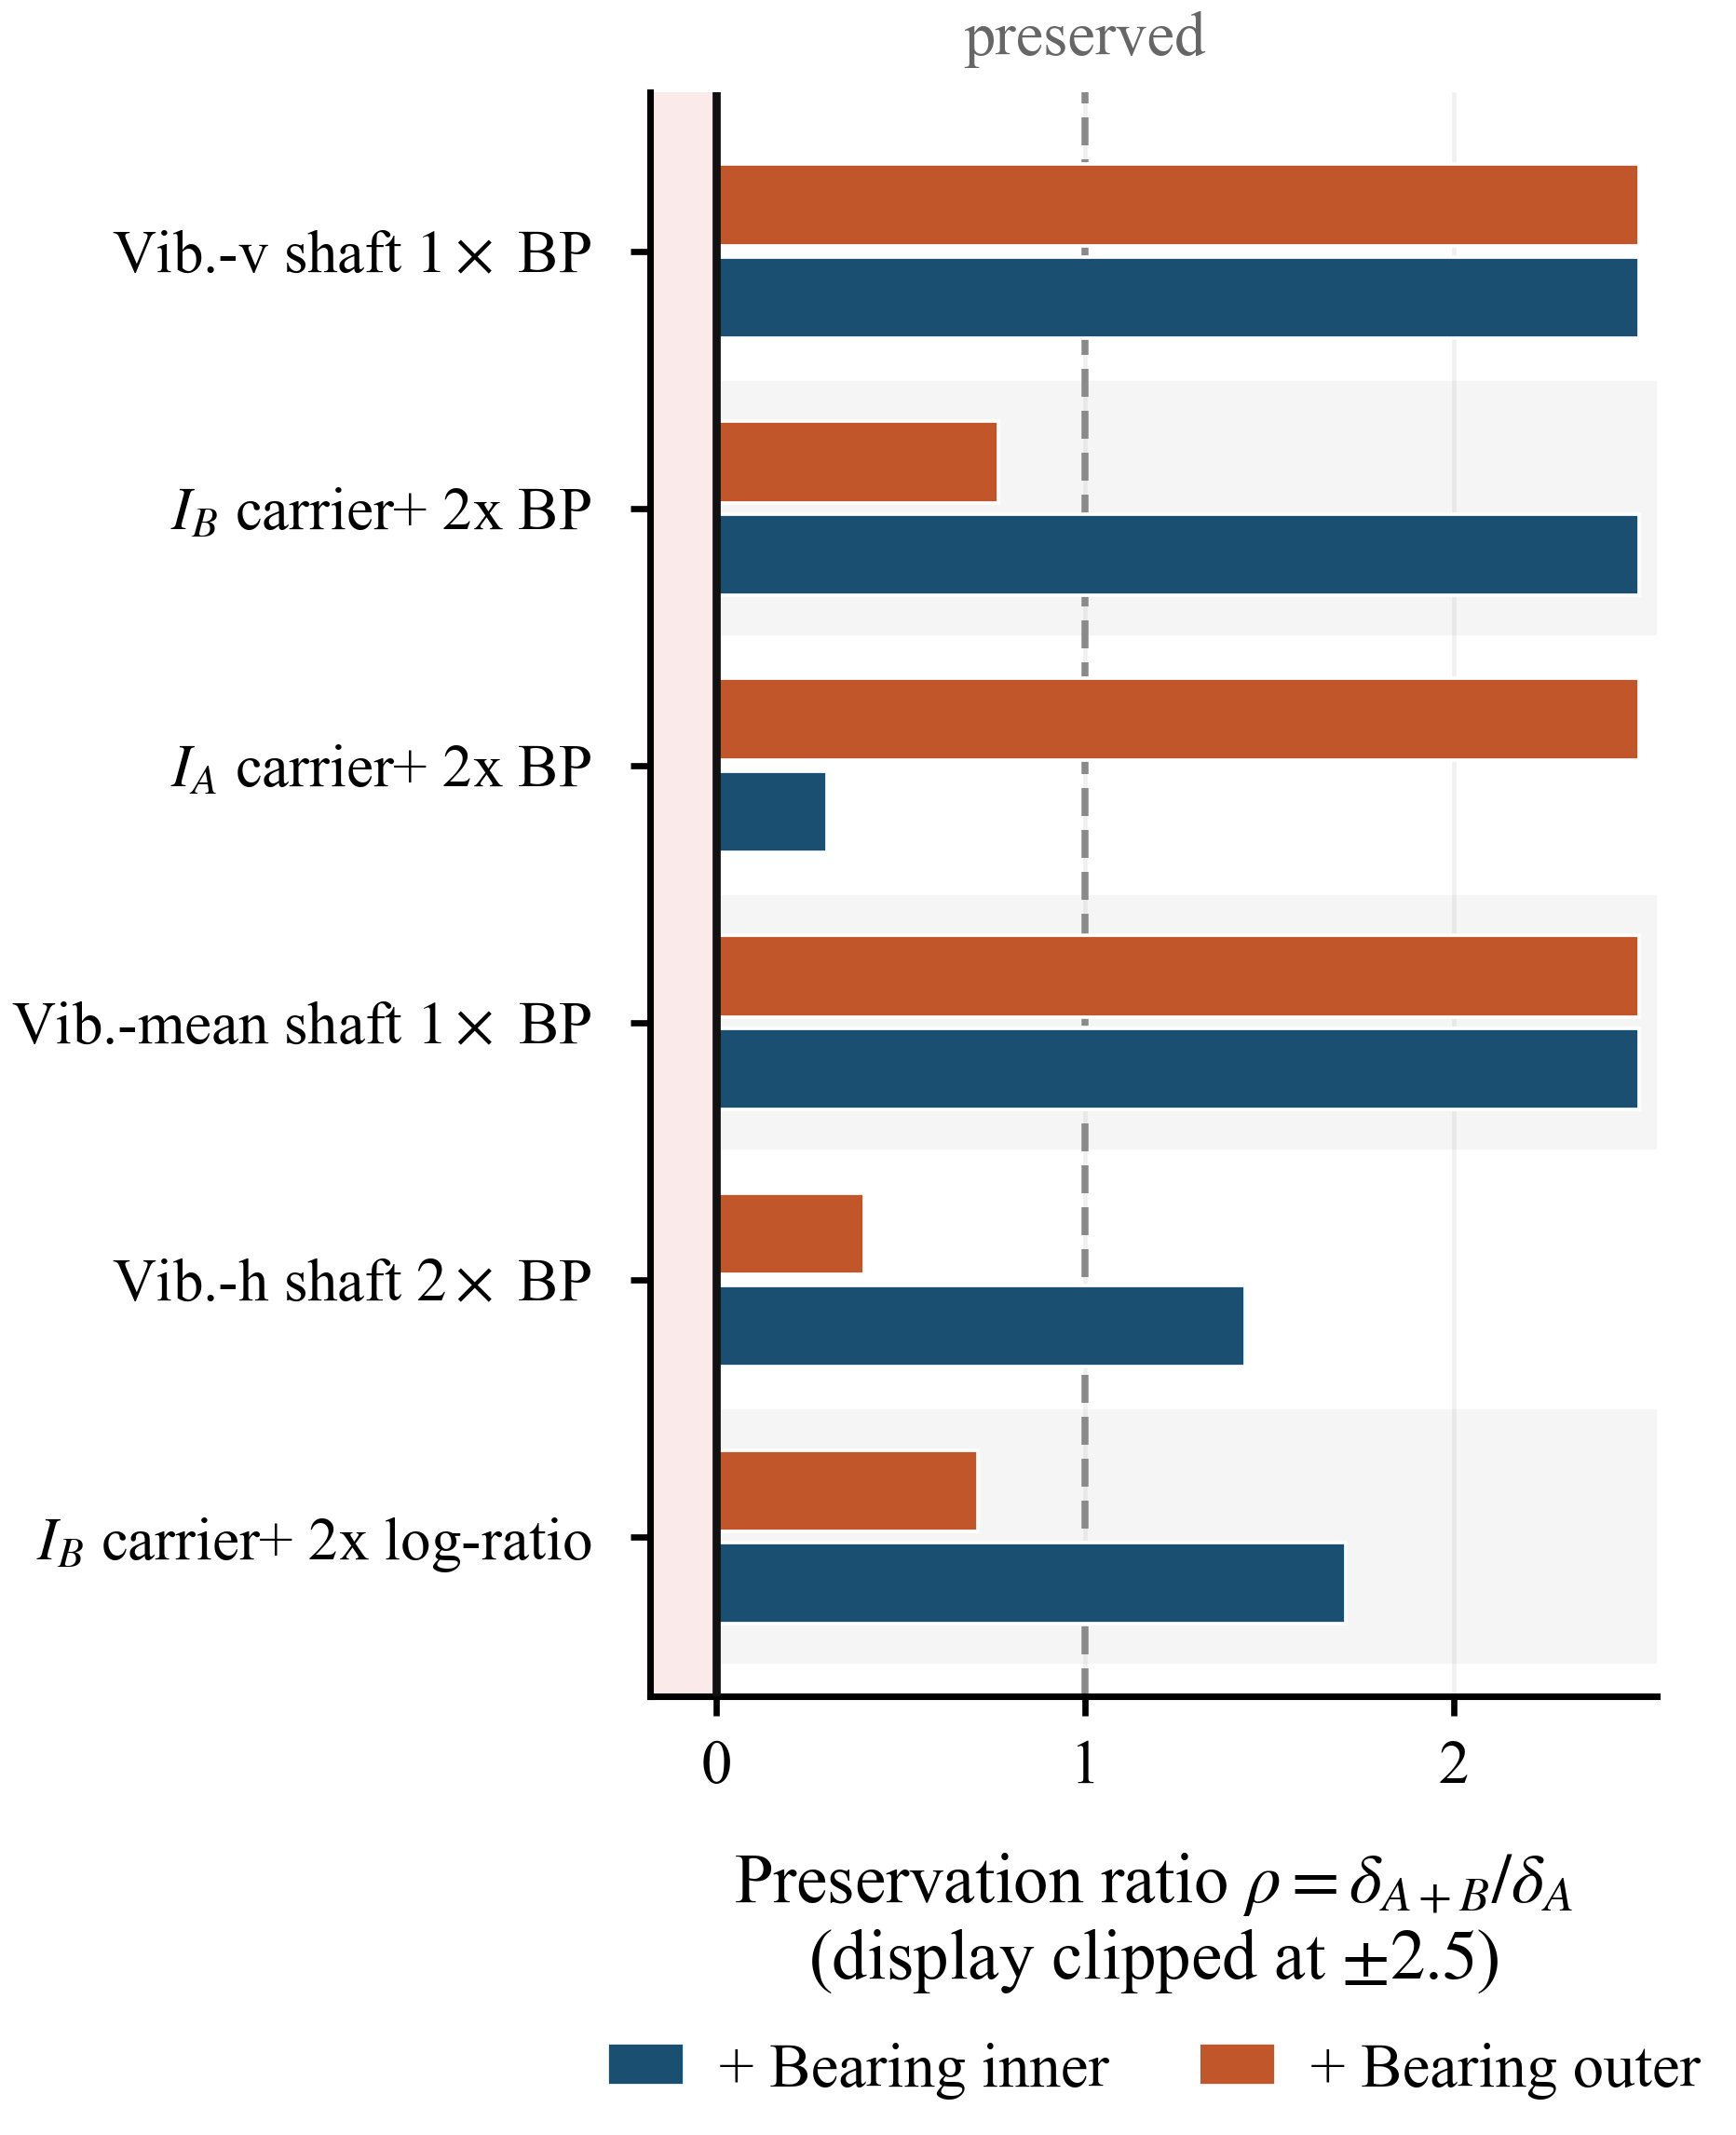
\includegraphics[width=\columnwidth]{fig5_preservation}
\caption{Feature-level preservation of selected static-eccentricity
signatures under bearing-inner and bearing-outer partner contexts. Negative
values indicate sign reversal, values near one preservation, and values
above one amplification.}
\label{fig:preservation}
\end{figure}

For the locked logistic-regression probe, the false-addition values in
Table~\ref{tab:crossed} should not be interpreted as conventional
false-alarm probabilities. The metric represents the mean number of
inactive constituent labels incorrectly activated per compound prediction.
Nevertheless, values of approximately 0.64--0.73 indicate a non-negligible
tendency toward over-diagnosis. In a practical condition monitoring system,
these additional constituent activations could increase inspection burden
even when one or both true mechanisms are successfully identified.
Deployment-oriented extensions should therefore consider cost-sensitive
threshold calibration or asymmetric decision penalties that explicitly
trade constituent recall against false additions. The classifier-family
robustness analysis further showed that this over-diagnosis tendency is not
fixed by the constituent representation itself: random forest and the
neural baseline reduced mean FA/run to approximately 0.26 while retaining
mean constituent recall near 0.66.

The observed cross-partner score reorientation also suggests a potential
role for representation or normalization strategies that explicitly promote
constituent consistency across compound contexts. Possible directions
include robust condition-aware normalization learned exclusively from
training data, partner-insensitive spectral reference schemes, or
representation constraints that align evidence for the same constituent
across different compound partners. However, the present preservation
analysis shows that the observed failure cannot be reduced to a uniform
inversion of the underlying physical features. Such adaptation strategies
should therefore be regarded as hypotheses for future investigation rather
than as established remedies for score-orientation reversal.

A further limitation is the recording structure of the public dataset.
Acquisition timestamps recovered from the released file names showed that
distinct recordings of the same fault state can be strongly separable in
the physics-feature space. Although same-date shared-partner controls
retained near-perfect discriminability, recording date is only a coarse
proxy for experimental session, and the available release does not provide
replicated same-state measurements sufficient to separate fault, assembly,
sensor-mounting, thermal, and recording-session effects. The cross-partner
results should therefore be interpreted as evidence of context-dependent
score transfer rather than as causal proof of physical signature inversion.
Absolute constituent-set reconstruction was additionally sensitive to the
classifier family: nonlinear tree and neural baselines substantially
reduced false additions and improved exact-match recovery, while the
descriptive advantage of recombination over complete compound-context
deprivation persisted across all four classifier families.

Taken together, the experiments identify two distinct limitations of
constituent-level compound-fault generalization. First, reduced
compound-context exposure became measurably detrimental when evaluation
also required generalization to an unseen operating condition. Second,
cross-partner transfer could be strongly directional even when within-pair
constituent evidence remained highly detectable. The latter included one
statistically supported case of complete score-orientation reversal, while
the available recording structure prevents attributing that reversal
uniquely to a physical signature inversion.

\section{Conclusion}
\label{sec:conclusion}

This paper evaluated whether the elementary mechanisms of a compound motor
fault can be recovered when their exact combination, their compound
context, and the operating condition are varied independently of the
training history. On a public multimodal induction-motor dataset whose
compound faults span mechanical and electrical modalities, a locked linear
constituent probe over mechanism-specific physical features showed that
strong closed-set discriminability (24-class accuracy 0.913, 95\% CI
$[0.885, 0.938]$) coexists with exact constituent-set recovery of only
0.083--0.157 on unseen compounds. The two results are not in tension; they
measure different abilities, and the gap between them is the paper's
subject.

Four conclusions follow from the controlled analyses. First, the failure
mode is incomplete decomposition rather than loss of information: at least
one true constituent was recovered in more than 92\% of compound runs, and
constituent recall (0.630--0.694) and all-constituent recovery under
recombination (up to 0.444) exceed input-independent prevalence references
(0.556 and 0.111, respectively), while several other partial-recovery
metrics do not---a distinction visible only because every metric was
reported against its constant-predictor floor. Second, compound-context
deprivation is measurably harmful chiefly when the operating condition is
simultaneously unseen: the recombination-versus-two-sided penalty under
condition shift was $+0.040$ micro-$F_1$ (95\% CI $[0.009, 0.073]$),
$+0.051$ constituent recall, and $+0.083$ all-constituent recovery, whereas
the corresponding seen-condition contrasts were not resolved. Third,
constituent evidence transfers across compound partners often but
directionally: within-pair detectability was near-perfect throughout, yet
cross-partner transfer ranged from perfect to a statistically supported
score-orientation reversal (Holm-adjusted $p \le 0.014$)---and the
demonstrated separability of distinct recordings of the same fault state
requires that reversal to be interpreted as context-dependent score
transfer rather than as proven physical signature inversion. Fourth,
absolute decomposition quality is an operating-point and model property:
precision-weighted thresholding raised exact-match recovery to
0.157--0.287 at reduced recall, and nonlinear classifier families reduced
false additions from ${\sim}0.68$ to ${\sim}0.26$ per run while the
qualitative generalization pattern persisted across all four families.

For practice, these results caution against reading closed-set accuracy as
deployment readiness, argue for calibrating constituent detectors with
explicit precision--recall cost structure, and indicate that commissioning
data should sample compound contexts and operating conditions jointly
rather than relying on either alone. The reference experiments of
Appendix~\ref{app:condition} reinforce the latter point: on this dataset
the standard leave-one-condition-out test is nearly saturated, while
single-condition training collapses accuracy, so robustness claims should
be evaluated in the extrapolating direction.

Several directions remain open. The dataset provides no replicated
same-state recordings that would separate fault, assembly, sensor-mounting,
and session effects, so the transfer analyses stop at carefully bounded
attribution; replicated acquisitions would convert those bounds into causal
statements. Representation or normalization strategies that promote
constituent-score consistency across compound partners are identified as
hypotheses, not established remedies. Finally, the constituent-level
protocol, prevalence references, and controls used here are directly
portable to the companion gearbox release and to other multimodal datasets,
where cross-dataset replication of the context-by-condition interaction
would test its generality.


\appendices
\section{Operating-Condition Reference Experiments}
\label{app:condition}

Section~\ref{sec:related} states that the leave-one-condition-out protocol,
the standard robustness test in the multi-condition literature, is nearly
saturated on this dataset, whereas the reverse direction is not. This
appendix reports the experiments behind that statement. They use a
deliberately generic pipeline---distinct from, and simpler than, the
constituent-level methodology of Section~\ref{sec:methods}---so that the
measured gaps reflect protocol difficulty rather than modeling choices, and
they are included with the released code.

Windows of 0.64~s (8192 samples, non-overlapping) were described by 108
time- and frequency-domain features (eight temporal statistics and ten
spectral descriptors per channel over the three vibration and three current
channels), classified into the original 24 diagnostic states by a 300-tree
random forest, with three seeds per configuration. Six split protocols were
compared. \emph{Random windows} splits windows irrespective of recording (a
deliberately leakage-prone reference); \emph{in-condition} trains on the
first 60\% of every recording and tests on the final 30\% with a 10\% guard
gap; \emph{unknown condition} holds out each of the twelve operating
conditions in turn; \emph{cross-profile} trains on one excitation profile
(constant-torque variable-speed or constant-speed variable-torque) and
tests on the other; \emph{steady~$\rightarrow$~transitional} trains on
quasi-stationary segments and tests on speed/load ramps, with stationarity
labeled from the key-phase-derived speed and the torque channel (the torque
channel is used only for this protocol construction and never as a
classifier input); and \emph{single source} inverts the unknown-condition
protocol, training on one condition and testing on the remaining eleven.

\begin{table}[!t]
\caption{Reference protocols, 24-class accuracy (mean $\pm$ std over folds
and three seeds). The same features and classifier are used throughout;
only the split changes.}
\label{tab:condref}
\centering
\footnotesize
\setlength{\tabcolsep}{5pt}
\begin{tabular}{l c c}
\toprule
Protocol & Folds & Accuracy \\
\midrule
Random windows (leakage-prone reference)   & 1  & $0.975 \pm 0.000$ \\
In-condition (guard-gap temporal split)    & 1  & $0.965 \pm 0.000$ \\
Unknown condition (leave-one-out)          & 12 & $0.939 \pm 0.024$ \\
Cross-profile                              & 2  & $0.839 \pm 0.115$ \\
Steady $\rightarrow$ transitional segments & 1  & $0.766 \pm 0.001$ \\
Single source (train on one condition)     & 12 & $0.333 \pm 0.104$ \\
\bottomrule
\end{tabular}
\end{table}

Table~\ref{tab:condref} summarizes the outcome. Holding one condition out
of twelve costs only ${\sim}2.6$ accuracy points relative to the
in-condition reference, because the eleven retained conditions bracket the
held-out one in speed and load and the model interpolates. Training on a
single condition and extrapolating to the other eleven costs over 60
points; paired over the twelve condition folds, the difference between the
two directions is 0.606 (paired $t$-test $p = 7.7\times10^{-10}$; Wilcoxon
$p = 4.9\times10^{-4}$). Transfer between excitation profiles is likewise
asymmetric at equal training size: training under variable speed
generalizes to variable load (accuracy 0.944), whereas the reverse loses
${\sim}21$ points (0.734; paired over seeds, $p = 3.3\times10^{-5}$).
Finally, appending 36 speed-invariant envelope-order descriptors to the
feature set leaves the interpolating protocols unchanged ($+0.001$ on
unknown-condition, paired $p = 0.84$) but significantly improves the
extrapolating one ($+0.047$ on single source, paired
$p = 8.4\times10^{-4}$), consistent with their construction.

Two implications carry into the main study. Methodologically, robustness to
operating conditions should be claimed in the extrapolating direction,
which motivates crossing the composition and context regimes with
unseen-condition evaluation rather than relying on leave-one-condition-out
alone. Practically, excitation diversity during commissioning matters more
than data volume: a training condition in which speed varies transfers to
load variation, but not conversely.


\section*{Data Availability}
The dataset analyzed in this study is publicly available from Mendeley Data
at \url{https://doi.org/10.17632/6s3dggj9mw.1} (CC~BY~4.0)
\cite{mcc5motor_data}, with its accompanying descriptor article
\cite{chen2026}. Acquisition-timestamp metadata used for the
recording-sensitivity controls were recovered from the released file names
and are included with the analysis code.

\section*{Code Availability}
The complete analysis code---including the constituent-level pipeline, the
crossed evaluation protocol, the constant-predictor references, the
recording-sensitivity controls, and the reference experiments of
Appendix~\ref{app:condition}---is available from the corresponding author
upon reasonable request.
% Stronger alternative for a paper about evaluation reliability: deposit the
% repository at Zenodo and cite its DOI here.

\bibliographystyle{IEEEtran}
\bibliography{refs}

\begin{IEEEbiography}[{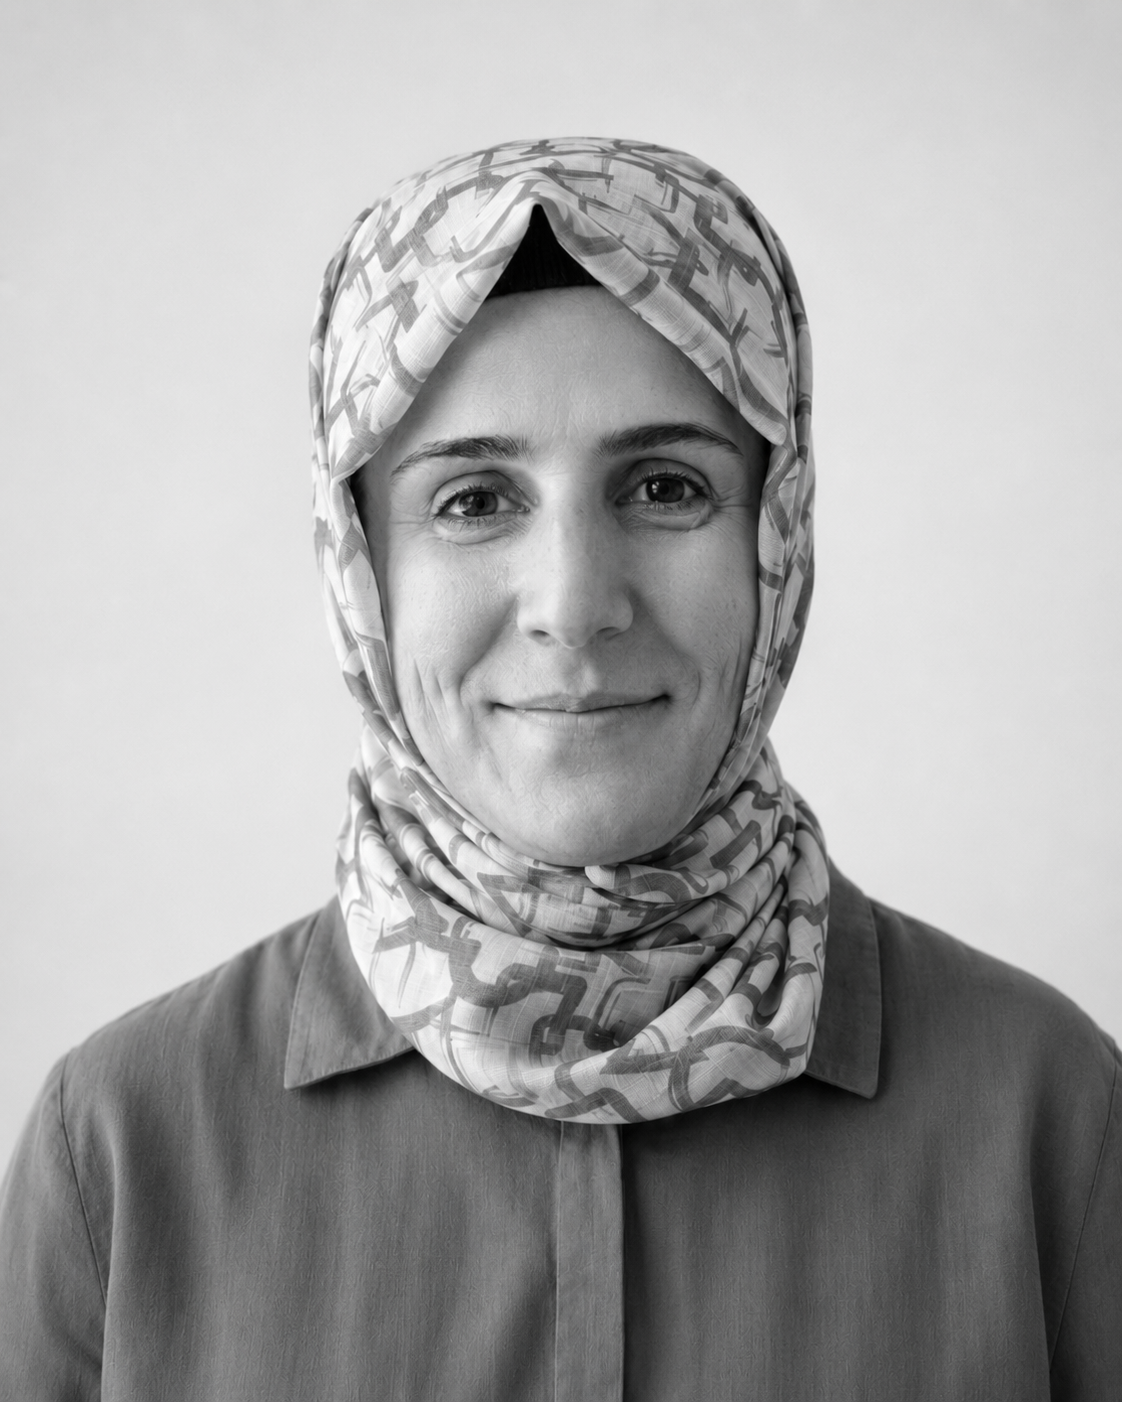
\includegraphics[width=1in,height=1.25in,clip,keepaspectratio]{photo_a}}]{Evin \c{S}ahin Sad{\i}k}
received the B.Sc. degree in Electrical and Electronics Engineering from
Bilecik \c{S}eyh Edebali University, Bilecik, Turkey, in 2012, and the
M.Sc. and Ph.D. degrees in Electrical and Electronics Engineering from
K\"utahya Dumlup{\i}nar University, K\"utahya, Turkey, in 2016 and 2022,
respectively. She is currently an Assistant Professor with the Department
of Electrical and Electronics Engineering, K\"utahya Dumlup{\i}nar
University. Her research interests include signal processing, machine
learning, and deep learning.
\end{IEEEbiography}

\begin{IEEEbiography}[{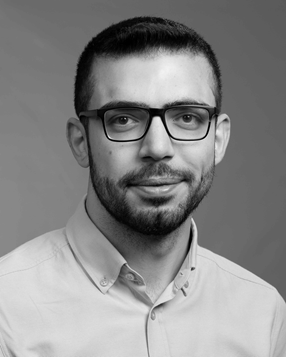
\includegraphics[width=1in,height=1.25in,clip,keepaspectratio]{photo_b}}]{H\"useyin Tayyer Canseven}
(Member, IEEE) received the B.Sc. and M.Sc. degrees in Electrical and
Electronics Engineering from Ege University, Izmir, Turkey, in 2018 and
2022, respectively, and the D.Sc. degree in Electrical Engineering from
Lappeenranta-Lahti University of Technology (LUT), Lappeenranta, Finland,
in 2025. He is currently a Post-Doctoral Researcher with the Department of
Electrical Engineering, LUT University. His research interests focus on
design and condition monitoring of electrical machines and motor drives.
\end{IEEEbiography}

\end{document}
